% Generated by GrindEQ Word-to-LaTeX 
\documentclass[subfooter]{deltares_manual}

\usepackage[english]{babel} %%% 'french', 'german', 'spanish', 'danish', etc.
\usepackage{amssymb}
\usepackage{amsmath}
\usepackage{txfonts}
\usepackage{mathdots}
\usepackage{caption}
\usepackage{float}
\usepackage{tikz}
\usetikzlibrary{arrows,quotes,positioning,shapes,calc}
\usepackage{algorithm}
\usepackage[noend]{algpseudocode}
%\usepackage[classicReIm]{kpfonts}
%\usepackage[dvips]{graphicx} %%% use 'pdftex' instead of 'dvips' for PDF output
\usepackage{pythonhighlight}
\usepackage{listings}

\tikzstyle{block} = [draw, fill=white, rectangle, 
minimum height=2em, minimum width=4em, node distance=6em]
\tikzstyle{round} = [draw, fill=white, circle,
minimum height=1em, minimum width=1em, node distance=6em]
\tikzstyle{input} = [coordinate]
\tikzstyle{output} = [coordinate]
\tikzstyle{pinstyle} = [pin edge={to-,thin,black}]

\svnid{$Id$}

%------------------------------------------------------------------------------
\hypersetup
{
	pdfauthor   = {Deltares},
	pdftitle    = {Probabilistic Toolkit Manual},
	pdfkeywords = {Probabilistic Toolkit},
	pdfcreator  = {LaTeX hyperref},
	pdfproducer = {ps2pdf}
}
%------------------------------------------------------------------------------


\begin{document}
	
\pagestyle{empty}

\title{Probabilistic Toolkit}
\subtitle{}
\manualtype{User Manual}
\version{2.0}
\manualtitle

\author{ }

\bibliographystyle{apalike}

%\deltarestitle	
	
\part{Introduction}

\chapter{Reading guide}

This document is a manual for the probabilistic toolkit. This document leads the user through a probabilistic analysis using the probabilistic toolkit. 

This document uses a number of examples. The examples are part of the Probabilistic Toolkit. They can be found in "$\text{Documents\textbackslash Deltares\textbackslash Probabilistic Toolkit}$" or, using the open dialog in the Probabilistic Toolkit, in the Probabilistic Toolkit section. 

\begin{figure}[H]
	\label{fig:Examples}
	\centering
	\includegraphics[scale=1.0]{pictures/examples.jpg}
	\caption{Examples}
\end{figure}


This document is split in a number of parts. They are:

\begin{itemize}
	\item Introduction: Contains some general information about the Probabilistic Toolkit.
	\item User Guide: Contains instruction how to use the Probabilistic Toolkit.
	\item Python interface: Contains instruction how to use the Probabilistic Toolkit functionality from Python.
	\item Scientific Background: Explains how calculations are performed.
\end{itemize}

\chapter{Introduction}

The probabilistic toolkit is able to perform probabilistic analyses on any model, ranging from python scripts to dedicated applications in the geotechnical or hydrodynamical field or to any other field to combinations of models.

The Probabilistic Toolkit offers a number of analysis types. They are performed in the order described in the next paragraph.

\section{Workflow}

The user should take a number of steps to perform a probabilistic analysis. These steps are 

\begin{enumerate}
	\item  Setting up the model (outside probabilistic toolkit)
	\item  Define the variables
	\item  Perform the probabilistic analysis. Possible analyses are:
	\begin{enumerate}
		\item  Run the model and compare results
		\item  Investigate the sensitivity of the model
		\item  Get input variables by calibation
		\item  Determine the output uncertainty
		\item  Determine the failure probability
	\end{enumerate}
\end{enumerate}

This is displayed in {\autoref{fig:WorkflowProbabilisticToolkit}}

\begin{figure}[H]
	\centering
	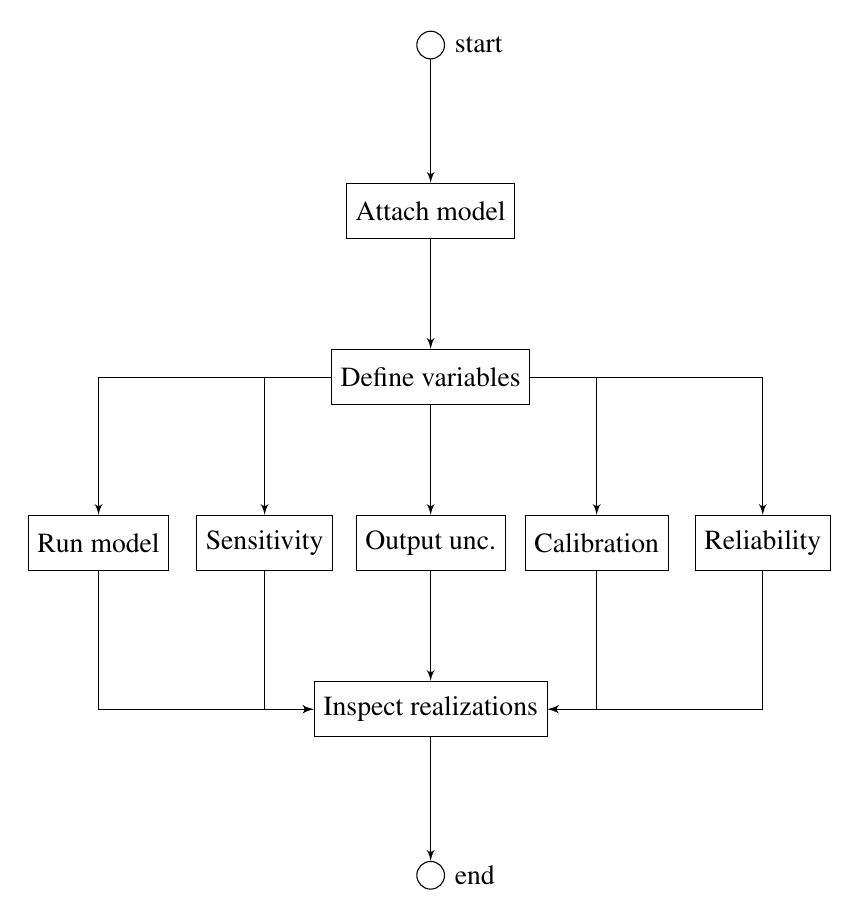
\begin{tikzpicture}[auto, node distance=2cm,>=latex']
	\node [round, label=east:start] (Start) {};
	\node [block, below of=Start] (Model) {Attach model};
	\node [block, below of=Model] (Variables) {Define variables};
	\node [block, below of=Variables] (BandWidth) {Output unc.};
	%\node [coordinate, below of=BandWidth] (C2) {};
	\node [block, left of=BandWidth] (Sensitivity) {Sensitivity};
	\node [block, left of=Sensitivity] (Run) {Run model};
	\node [block, right of=BandWidth] (Calibration) {Calibration};
	\node [block, right of=Calibration] (Failure) {Reliability};
	\node [block, below of=BandWidth] (Calculations) {Inspect realizations};
	\node [round, below of=Calculations, label=east:end] (End) {};
	
	\draw [->] (Start) -- (Model);
	\draw [->] (Model) -- (Variables);
	\draw [->] (Variables) -| (Run);
	\draw [->] (Variables) -| (Sensitivity);
	\draw [->] (Variables) -- (BandWidth);
	\draw [->] (Variables) -| (Calibration);
	\draw [->] (Variables) -| (Failure);
	\draw [->] (Run) |- (Calculations);
	\draw [->] (Sensitivity) |- (Calculations);
	\draw [->] (BandWidth) -- (Calculations);
	\draw [->] (Failure) |- (Calculations);
	\draw [->] (Calibration) |- (Calculations);
	\draw [->] (Calculations) -- (End);
	
	\end{tikzpicture}
	\caption{Workflow through probabilistic toolkit}
	\label{fig:WorkflowProbabilisticToolkit}
\end{figure}

The workflow sequence is reflected by the tabs in the main tab control of the application. Depending on the selected analysis type, model and calculation options the visible tabs may change a bit.

\begin{figure}[H]
	\label{fig:WorkflowTabs}
	\centering
	\includegraphics[scale=1.0]{pictures/workflow-tabs.jpg}
	\caption{Workflow tabs}
\end{figure}

The order of the steps 'Attach model', 'Define variables' and 'Perform analysis' is fixed, although one can always return to a previous step. The steps within the step 'Perform analysis', which are 'Run model', 'Sensitivity', 'Output uncertainty', 'Calibration' and 'Reliability' are optional and can be performed in any order.

\section{Run Model}

Running a model is the most simple application in the Probabilistic Toolkit. It just, as the word says, runs a model and displays its results. This can be done for one input set or for several input sets, where one or more parameters are varied.

Running a model helps the user to get a feel for the model and check whether the model has been attached to the Probabilistic Toolkit in the right way. See \autoref{ug:RunModel} for more information.

\section{Sensitivity}

In sensitivity analysis the effects of changes to input variables are investigated. 

This will give insight in which input parameters are important and help the user decide which input parameters must be measured more precisely. See \autoref{ug:Sensitivity} for more information.

\section{Output uncertainty}

Output uncertainty is an extension of sensitivity analysis. Now all input parameters are varied according to their uncertainty definition. This leads to uncertainty of the output parameters.

This is useful when the user is interested in possible values in the future of a physical property. For example, due to a load subsidence of the soil surface will occur. It is interesting how much subsidence will occur in the next ten years. Another example, due to a side stream a gully will move sidewards. It is interesting to know the location of the gully in the next year.

See \autoref{ug:OutputUncertainty} for more information.

\section{Calibration}

Calibration is a method where input parameters can be derived from measured output parameters, including uncertainty. Calibration can be used to obtain parameters, which are difficult to obtain directly.

For example, the roughness of a river bed is hard to obtain. Using measured values such as time series of water levels at different locations, the roughness coefficients are determined. 

See \autoref{ug:Calibration} for more information.

\section{Reliability}

Reliabiity analysis determines the reliability, or probability of failure, of a physical construction. This gives the user insight of the probabilty that an unwanted phenomenon will happen, possibly within a given period of time. 

For example, the probability that a dike will fail can be calculated. This is used in assessment of dikes and using this probability, a decision will be made to strengthen it. An accurate calculation of the probability of failure is important, since it can save money by not strengthening it more than necessary.

To calculate an accurate probability of failure, survived situations can be used. Even lots of effort have been put in measuring input values, it is impossible to know the subsoil in long stretches of dikes completely. So it might be possible that a model predicts dike failure, while in reality it has been observed that the dike has survived. The Probabilistic Toolkit uses these events to update the probability of failure.

Another example is risk based asset management. In risk based asset management a maintenance schedule will be set up, so that total costs over a long period are minimal. The total costs include strengthening actions and risk (risk is probability times damage).

See \autoref{ug:Reliability} for more information.

\begin{figure}[H]
	\label{fig:HighWaterLevel}
	\centering
	\includegraphics[width=0.8\textwidth]{pictures/dike.png}
	\caption{High water level}
\end{figure}

\chapter{Run}

The Probabilistic Toolkit supports the following ways of running a probabilistic analysis:

\section{Application}

The Probabilistic toolkit should be started with its user interface, which can be found in the start menu or as icon on the desktop. Then the user can enter all data required by the workflow and execute the run button. All data and results be saved and later opened again from a tkx-file. 

\section{Console}
\label{sec:Console}

The console version enables execution of a probabilistic analysis without user interface. An input file should be available (made with the user interface). The console version performs the calculation as specified in the input file. 

The console application should be run as follows:

\begin{lstlisting}[language=sh, basicstyle=\ttfamily, frame=single]
Deltares.Probabilistic.Console.exe input.tkx [output.tkx]
\end{lstlisting}

If no output file is specified, the input file is used and overwritten as the file containing the calculation results.

\section{Python}

Using Python, the input file of the Probabilistic Toolkit can be modified and run (only for reliability analysis). The Probabilistic Toolkit installs a python file, named toolkit.py, by which properties in an existing toolkit file can be modified and run. This file is located in the sub directory Python of the installation directory (usually C:/Program Files (x86)/Deltares/Probabilistic toolkit/Python).

See \autoref{ug:PythonInterface} for more information.


\part{Python interface}

\chapter{Python interface}
\label{ug:PythonInterface}

\section{Run python scripts}

The Probablistic Toolkit provides a python model, by which modifications can be made to a project file and runs can be made. This file is toolkit\_model.py is installed in the subdirectory Python of the installation directory of the Probabilistic Toolkit.

Python scripts can be run in two ways: Python is in control or the Probablistic Toolkit is in control

\subsection{Python in control}

In this way Python is the process which is started initially. The Python process makes connection to the Probabilistic Toolkit. Such a process consists of the following steps:

\begin{enumerate}
	\item Establish connection with the Probabilistic Toolkit;
	\item Load an input file (*.tkx), internally the contents of the file become available as a project
	\item Make changes to the project
	\item Run the calculation
	\item Retrieve the results of the calculation
	\item Save the results in a file (*.tkx)
	\item Disconnect from the Probablistic Toolkit
\end{enumerate}

This is coded as follows: 

\begin{lstlisting}[language=Python, basicstyle=\ttfamily, frame=single]
import sys
sys.path.append('<installdir>\Python')

from toolkit_model import *

# make connection to the Probabilistic Toolkit
toolkit = ToolKit()

# load an input file 
project = toolkit.load('example.tkx')

# make changes to the project, for example modify the settings
project.settings.method = 'FORM'
project.settings.relaxation_factor = 0.25

# validate and run if ok
messages = project.validate()
if len(messages) == 0:
	project.run()

# do something with the results, 
# for example print the reliabilty index
reliability_index = project.design_point.reliability_index
print('reliability index = ' + str(reliability_index))

# save the results
toolkit.save('example.tkx')

# disconnected when the toolkit object is garbage collected
\end{lstlisting}

\subsection{Toolkit in control}
\label{sec:PythonToolkitControl}

When the Probablistic Toolkit is started, it can run a python process before and after the calculation, see \autoref{sec:PrePostProcessing}. The connection with the toolkit is provided automatically and the project available in the toolkit is loaded already. The path to  toolkit\_model.py is set allready.

A preprocessor has in general the following structure:

\begin{enumerate}
	\item Connect to the project
	\item Make changes to the project
\end{enumerate}

In code a preprocessor will look as follows:
\begin{lstlisting}[language=Python, basicstyle=\ttfamily, frame=single]
from toolkit_model import *

# connect to the project
project = Project()

# do something with project, for example
# change one of the distributions to a fragility curve
h = project.model.get_variable('h')
h.clear()

h.set_fragility_prob_failure(1.5, 4.3)
h.set_fragility_prob_failure(2.8, 2,5)
\end{lstlisting}

After execution of this script, the Probablistic Toolkit will perform the calculation. Then a postprocessor can be invoked. A postprocessor will have the following structure:

\begin{enumerate}
	\item Connect to the project
	\item Retrieve the results of the calculation
\end{enumerate}

In code a postprocessor will look as follows:
\begin{lstlisting}[language=Python, basicstyle=\ttfamily, frame=single]
from toolkit_model import *

# connect to the project
project = Project()

# do something with the results, 
# for example print the reliabilty index
reliability_index = project.design_point.reliability_index
print('reliability index = ' + str(reliability_index))
\end{lstlisting}

or, when an output uncertainty calcualtion is made:

\begin{lstlisting}[language=Python, basicstyle=\ttfamily, frame=single]
import os
import sys
from toolkit_model import *

# argument for export file must be given
export_file = os.path.abspath(sys.argv[1])

project = Project()

lines = []

for var in project.model.response_variables:
	var = project.get_uncertainty_variable(var)
	lines.append("{0};{1};{2};{3}\n".format(
	  var.name,
	  var.get_quantile(0.1),
	  var.get_quantile(0.5),
	  var.get_quantile(0.9)))

with open(export_file, 'w') as f:
	f.writelines(lines)
\end{lstlisting}



\section{Reference}

The following methods are available:

\subsection{Class ToolKit}

The ToolKit class is only needed when Python is in control of the whole process. The Toolkit class should never be used in a preprocessor or postprocessor. The purpose of the class is to establish an connection with the Probabilistic Toolkit, loading a project and saving a project.

\begin{longtable*}{p{20mm}p{\textwidth-24pt-20mm}}  
	Constructor & \\
	Functionality & Establishes a connection with the Probablistic Toolkit; \\  
	Arguments & None; \\  
\end{longtable*}

\begin{longtable*}{p{20mm}p{\textwidth-24pt-20mm}}  
	Finalizer & \\
	Functionality & Disconnects from the Probablistic Toolkit; \\  
\end{longtable*}

\begin{longtable*}{p{20mm}p{\textwidth-24pt-20mm}}  
	Method &  \textbf{load}\\
	Functionality & Loads a project. All subsequent operations are applied on this project. Only one project can be loaded at a time; \\  
	Arguments & full path to *.tkx file; \\  
	Returns & Project; \\  
\end{longtable*}

\begin{longtable*}{p{20mm}p{\textwidth-24pt-20mm}}  
	Method &  \textbf{save}\\
	Functionality & Saves the current project; \\  
	Arguments & full path to *.tkx file; \\  
	Returns & Nothing; \\  
\end{longtable*}

\begin{longtable*}{p{20mm}p{\textwidth-24pt-20mm}}  
	Method &  \textbf{exit}\\
	Functionality & Optional method to stop the background server, which takes care for handling all commands. This call should not be necessary, since it is invoked automatically in the Finalizer. \\  
	Arguments & None; \\  
	Returns & Nothing; \\  
\end{longtable*}

\subsection{Class Project}

The Project class contains all input data and results of a project. It contains the methods to start the calculation.

\begin{longtable*}{p{20mm}p{\textwidth-24pt-20mm}}  
	Constructor & \\
	Functionality & Creates a project referencing the current project in the Probabilistic Toolkit. Only call the constructor if python is called in the preproocessor or postprocessor, otherwise use the load method in the class ToolKit; \\  
	Arguments & None; \\  
\end{longtable*}

\begin{longtable*}{p{20mm}p{\textwidth-24pt-20mm}}  
	Method &  \textbf{validate}\\
	Functionality & Validates the project; \\  
	Arguments & Nothing; \\  
	Returns & List of strings containng error validation messages; \\  
\end{longtable*}

\begin{longtable*}{p{20mm}p{\textwidth-24pt-20mm}}  
	Method &  \textbf{run}\\
	Functionality & Runs the calculation and waits until the calculation has finished. Do not call this method in a preprocessor or postprocessor; \\  
	Arguments & Nothing; \\  
	Returns & Indicator 'ok' or 'failed'; \\  
\end{longtable*}

\begin{longtable*}{p{20mm}p{\textwidth-24pt-20mm}}  
	Property &  \textbf{model}\\
	Functionality & Gets the model instance; \\  
	Type & Model; \\  
\end{longtable*}

\begin{longtable*}{p{20mm}p{\textwidth-24pt-20mm}}  
	Property &  \textbf{settings}\\
	Functionality & Gets an object containing all settings; \\  
	Type & Settings; \\  
\end{longtable*}

\begin{longtable*}{p{20mm}p{\textwidth-24pt-20mm}}  
	Property &  \textbf{identifier}\\
	Functionality & Gets or sets the identifier used in \autoref{sec:PrePostProcessing}; \\  
	Type & Model; \\  
\end{longtable*}

\begin{longtable*}{p{20mm}p{\textwidth-24pt-20mm}}  
	Property &  \textbf{uncertainty\_variable}\\
	Functionality & Gets the first uncertainty variable; \\  
	Type & UncertaintyStochast; \\  
\end{longtable*}

\begin{longtable*}{p{20mm}p{\textwidth-24pt-20mm}}  
	Method &  \textbf{get\_uncertainty\_variable}\\
	Functionality & Gets the uncertainty variable with a given name; \\  
	Arguments & string or ResponseStochast; \\  
	Returns & UncertaintyStochast; \\  
\end{longtable*}

\begin{longtable*}{p{20mm}p{\textwidth-24pt-20mm}}  
	Property &  \textbf{uncertainty\_variables}\\
	Functionality & Gets all resulting uncertainty variables; \\  
	Type & List of UncertaintyStochast; \\  
\end{longtable*}

\begin{longtable*}{p{20mm}p{\textwidth-24pt-20mm}}  
	Property &  \textbf{design\_point}\\
	Functionality & Gets the result of a reliability calculation; \\  
	Type & DesignPoint; \\  
\end{longtable*}

\begin{longtable*}{p{20mm}p{\textwidth-24pt-20mm}}  
	Property &  \textbf{design\_points}\\
	Functionality & Gets all resulting design points; \\  
	Type & List of DesignPoints; \\  
\end{longtable*}

\begin{longtable*}{p{20mm}p{\textwidth-24pt-20mm}}  
	Property &  \textbf{realizations}\\
	Functionality & Gets all realizations; \\  
	Type & List of Realizations; \\  
\end{longtable*}

\subsection{Class Model}

The Model class contains all input data. Do not create a Model, but use the Project.model property.

\begin{longtable*}{p{20mm}p{\textwidth-24pt-20mm}}  
	Property & \textbf{input\_file}\\
	Functionality & Gets or sets the input file name of a file based model; \\  
	Type & string (full path); \\  
\end{longtable*}

\begin{longtable*}{p{20mm}p{\textwidth-24pt-20mm}}  
	Property &  \textbf{submodels}\\
	Functionality & Gets a list of all sub models in case of a composite model; \\  
	Type & string (full path); \\  
\end{longtable*}

\begin{longtable*}{p{20mm}p{\textwidth-24pt-20mm}}  
	Method &  \textbf{get\_submodel}\\
	Functionality & Gets the submodel with a specified name; \\  
	Arguments & name of variable; \\  
	Returns & SubModel or None if not found; \\  
\end{longtable*}

\begin{longtable*}{p{20mm}p{\textwidth-24pt-20mm}}  
	Property &  \textbf{variables}\\
	Functionality & Gets a list of all variables; \\  
	Type & array of strings; \\  
\end{longtable*}

\begin{longtable*}{p{20mm}p{\textwidth-24pt-20mm}}  
	Method &  \textbf{get\_variable}\\
	Functionality & Gets the variable with a specified full name of the variable (name including model name if the model is a composite model); \\  
	Arguments & name of variable; \\  
	Returns & Stochast or None if not found; \\  
\end{longtable*}

\begin{longtable*}{p{20mm}p{\textwidth-24pt-20mm}}  
	Property &  \textbf{response\_variables}\\
	Functionality & Gets a list of all response variables; \\  
	Type & string (full path); \\  
\end{longtable*}

\begin{longtable*}{p{20mm}p{\textwidth-24pt-20mm}}  
	Method &  \textbf{get\_response\_variable}\\
	Functionality & Gets the response variable with a specified name; \\  
	Arguments & name of variable; \\  
	Returns & ResponseStochast or None if not found; \\  
\end{longtable*}

\begin{longtable*}{p{20mm}p{\textwidth-24pt-20mm}}  
	Method &  \textbf{run}\\
	Functionality & Runs the model with the input file specified for this model. This might be necessary to generate the output values in the output file, which is necessary for the Probabilistic Toolkit to perform an project.run(); \\  
	Arguments & None; \\  
	Returns & Nothing; \\  
\end{longtable*}

\subsection{Class SubModel}

The SubModel class contains input data of a sub model. Do not create this class.

\begin{longtable*}{p{20mm}p{\textwidth-24pt-20mm}}  
	Property &  \textbf{input\_file}\\
	Functionality & Gets or sets the input file name of a file based model; \\  
	Type & string (full path); \\  
\end{longtable*}

\begin{longtable*}{p{20mm}p{\textwidth-24pt-20mm}}  
	Method &  \textbf{run}\\
	Functionality & Runs the model with the specified for this submodel. This might be necessary to generate the output values in the output file, which is necessary for the Probabilistic Toolkit to perform an project.run(); \\  
	Arguments & None; \\  
	Returns & Nothing; \\  
\end{longtable*}

\subsection{Class Stochast}

The Stochast class contains all properties of a variable.

\begin{longtable*}{p{20mm}p{\textwidth-24pt-20mm}}  
	Property &  \textbf{name}\\
	Functionality & Gets the name of the variable; \\  
	Type & string; \\  
\end{longtable*}

\begin{longtable*}{p{20mm}p{\textwidth-24pt-20mm}}  
	Property &  \textbf{fullname}\\
	Functionality & If the model is a composite model, gets the model name and variable name, else gets the variable name; \\  
	Type & string; \\  
\end{longtable*}

\begin{longtable*}{p{20mm}p{\textwidth-24pt-20mm}}  
	Property &  \textbf{distribution}\\
	Functionality & Gets or sets the distribution type, one of:  Deterministic, Normal, LogNormal, StudentT, Uniform, Triangular, Trapezoidal, Exponential, Gamma, Beta, Frechet, Weibull, Gumbel, GeneralizedExtremeValue, Rayleigh, Pareto, GeneralisedPareto, Table (= histogram), Discrete, Poisson, FragilityCurve). The distribution type is not case sensitive; \\  
	Type & string; \\  
\end{longtable*}

\begin{longtable*}{p{20mm}p{\textwidth-24pt-20mm}}  
	Properties &  \textbf{mean, deviation, variation, minimum, maximum, shift, shift\_b, rate, shape, shape\_b, location, scale, observations, design\_fraction, design\_factor}\\
	Functionality & Gets or sets the property of a variable. Deviation refers to standard deviation and variation refers to variation coefficient; \\  
	Type & float; \\  
\end{longtable*}

\begin{longtable*}{p{20mm}p{\textwidth-24pt-20mm}}  
	Method & \textbf{get\_quantile}\\
	Functionality & Gets the value belonging to a given quantile; \\  
	Arguments & Quantile; \\  
	Returns & Value at quantile; \\  
\end{longtable*}

\begin{longtable*}{p{20mm}p{\textwidth-24pt-20mm}}  
	Method & \textbf{get\_design\_value}\\
	Functionality & Gets the design value; \\  
	Arguments & None; \\  
	Returns & Value based on design\_fraction and design\_factor; \\  
\end{longtable*}

\begin{longtable*}{p{20mm}p{\textwidth-24pt-20mm}}  
	Method &  \textbf{clear}\\
	Functionality & Resets the distribution type to deterministic and removes all fragility values, discrete values and histogram bins; \\  
	Arguments & None; \\  
	Returns & Nothing; \\  
\end{longtable*}

\begin{longtable*}{p{20mm}p{\textwidth-24pt-20mm}}  
	Methods & \textbf{set\_fragility\_reliability\_index, set\_fragility\_prob\_failure, set\_fragility\_prob\_non\_failure} \\
	Functionality & Adds or updates a fragility value of a variable which has distribution type fragility curve; \\  
	Arguments & Variable name; \\  
	& Value of the conditional variable; \\
	& Reliability index, probabilty of failure or non failure at the value of the conditional variable; \\
	Returns & Nothing; \\  
\end{longtable*}

\begin{longtable*}{p{20mm}p{\textwidth-24pt-20mm}}  
	Method & \textbf{set\_fragility\_reliability\_index} \\
	Functionality & Adds or updates a fragility value of a variable which has distribution type fragility curve; \\  
	Arguments & Variable name; \\  
	& Value of the conditional variable; \\
	& Reliability index at the value of the conditional variable; \\
	Returns & Nothing; \\  
\end{longtable*}

\begin{longtable*}{p{20mm}p{\textwidth-24pt-20mm}}  
	Method & \textbf{set\_discrete\_value} \\
	Functionality & Adds or updates a discrete value of a variable which has distribution type discrete; \\  
	Arguments & Variable name; \\  
	& Value of the conditional variable; \\
	& Occurrences at the value of the conditional variable; \\
	Returns & Nothing; \\  
\end{longtable*}

\begin{longtable*}{p{20mm}p{\textwidth-24pt-20mm}}  
	Method & \textbf{set\_histogram\_value} \\
	Functionality & Adds a bin of a variable which has distribution type histogram; \\  
	Arguments & Variable name; \\  
	& Lower boundary of the bin; \\
	& Upper boundary of the bin; \\
	& Numer of occurences in the bin; \\
	Returns & Nothing; \\  
\end{longtable*}

\begin{longtable*}{p{20mm}p{\textwidth-24pt-20mm}}  
	Methods & \textbf{get\_correlation, set\_correlation} \\
	Functionality & Gets or sest the correlation between two variables; \\  
	Arguments & Other variable name; \\
	& set: new correlation value\\  
	Returns & get: Correlation, set: Nothing; \\  
\end{longtable*}

\subsection{Class ResponseStochast}

The Stochast class contains all properties of a response variable.

\begin{longtable*}{p{20mm}p{\textwidth-24pt-20mm}}  
	Property &  \textbf{name}\\
	Functionality & Gets the name of the response variable; \\  
	Type & string; \\  
\end{longtable*}

\begin{longtable*}{p{20mm}p{\textwidth-24pt-20mm}}  
	Property &  \textbf{fullname}\\
	Functionality & Gets the full name (name including model if the model is a composite model) of the response variable; \\  
	Type & string; \\  
\end{longtable*}

\subsection{Class Settings}

The Settings class contains computational settings.

\begin{longtable*}{p{20mm}p{\textwidth-24pt-20mm}}  
	Property & \textbf{method} \\
	Functionality & Gets or sets the calculation method; \\  
	Type & Calculation method (one of: NumericalIntegration, NumericalBisection, MonteCarlo, LatinHyperCube, DirectionalSampling, ImportanceSampling, SubsetSimulation, Cobyla, FORM, FOSM, FragilityCurveIntegration, 	Experimental). The calculation method is not case sensitive; \\  
\end{longtable*}

\begin{longtable*}{p{20mm}p{\textwidth-24pt-20mm}}  
	Property & \textbf{start\_method} \\
	Functionality & Sets the calculation start method; \\  
	Type & Calculation start method (one of: None, RaySearch, SensitivitySearch, SphereSearch). The calculation start method is not case sensitive; \\  
\end{longtable*}

\begin{longtable*}{p{20mm}p{\textwidth-24pt-20mm}}  
	Properties & \textbf{minimum\_samples, maximum\_samples, minimum\_iterations, maximum\_iterations, relaxation\_factor, relaxation\_loops, variation\_coefficient\_failure, intervals, variance\_factor, start\_value, variance\_loops,	min\_variance\_loops, fraction\_failed} \\
	Functionality & Gets or sets a settings value; \\  
	Type & float\\  
\end{longtable*}

\begin{longtable*}{p{20mm}p{\textwidth-24pt-20mm}}  
	Method & \textbf{get\_variable\_settings} \\
	Functionality & Gets an object containing calculation settings of a variable; \\  
	Arguments & Variable name; \\  
	Returns & StochastSettings; \\  
\end{longtable*}

\subsection{Class StochastSettings}

The StochastSettings class contains computational settings of a variable

\begin{longtable*}{p{20mm}p{\textwidth-24pt-20mm}}  
	Property & \textbf{name} \\
	Functionality & Gets the variable name; \\  
	Type & string; \\  
\end{longtable*}

\begin{longtable*}{p{20mm}p{\textwidth-24pt-20mm}}  
	Property & \textbf{start\_value} \\
	Functionality & Gets or sets the start value; \\  
	Type & float; \\  
\end{longtable*}

\subsection{Class UncertaintyStochast}

The DesignPoint class contains the result of a reliabliity calculation

\begin{longtable*}{p{20mm}p{\textwidth-24pt-20mm}}  
	Property & \textbf{name} \\
	Functionality & Gets the name of the reponse variable; \\  
	Type & string; \\  
\end{longtable*}

\begin{longtable*}{p{20mm}p{\textwidth-24pt-20mm}}  
	Method & \textbf{get\_quantile} \\
	Functionality & Gets the quantile of the uncertainty variable; \\  
	Arguments & Quantile; \\  
	Returns & Value at quantile; \\  
\end{longtable*}


\subsection{Class DesignPoint}

The DesignPoint class contains the result of a reliabliity calculation

\begin{longtable*}{p{20mm}p{\textwidth-24pt-20mm}}  
	Property & \textbf{identifier} \\
	Functionality & Gets the numeric identifier of the design point, for example the varing parameters in a table scenario; \\  
	Type & array of floats; \\  
\end{longtable*}

\begin{longtable*}{p{20mm}p{\textwidth-24pt-20mm}}  
	Properties & \textbf{reliability\_index, probability\_failure, convergence} \\
	Functionality & Gets the result values of the reliability calculation; \\  
	Type & float; \\  
\end{longtable*}

\begin{longtable*}{p{20mm}p{\textwidth-24pt-20mm}}  
	Method & \textbf{get\_alpha} \\
	Functionality & Gets the contribution of a variable to the design point; \\  
	Arguments & Variable full name or ResponseStochast; \\  
	Returns & Alpha; \\  
\end{longtable*}

\begin{longtable*}{p{20mm}p{\textwidth-24pt-20mm}}  
	Property & \textbf{realizations} \\
	Functionality & Gets the realizations needed to calculate the design point; \\  
	Type & List of Realizations; \\  
\end{longtable*}

\subsection{Class Alpha}

\begin{longtable*}{p{20mm}p{\textwidth-24pt-20mm}}  
	Properties & \textbf{alpha\_value, physical\_value} \\
	Functionality & Gets the result values of the contribution to the design point; \\  
	Type & float; \\  
\end{longtable*}

\subsection{Class Realization}

\begin{longtable*}{p{20mm}p{\textwidth-24pt-20mm}}  
	Properties & \textbf{z, weight, beta} \\
	Functionality & Gets the limit state, weight and beta of the realization; \\  
	Type & float; \\  
\end{longtable*}

\begin{longtable*}{p{20mm}p{\textwidth-24pt-20mm}}  
	Method & \textbf{get\_value} \\
	Functionality & Gets the value of a variable (input or response) in the realization; \\  
	Arguments & Full name of the variable; \\  
	Returns & Value of the stochastic variable in the realization; \\  
\end{longtable*}


\part{Scientific Background}

\chapter{Distributions}

\section{Standard normal distribution}

The standard normal distribution is a normal distribution with mean $\mu$ = 0 and deviation $\sigma$ = 1. The standard normal distribution is unlikely to occur in the real world, but is used internally in probabilistic calculations.

The probability density function is

\begin{align}
\label{eq:StandardNormalPDF}
\varphi\left(u\right)= \frac{1}{\sqrt{2\pi}} e^{-u^{2} / 2} 
\end{align} 

and the cumulative density function, or in other words the non exceeding probability, is

\begin{align}
\label{eq:StandardNormalCDF}
\Phi\left(u\right) = \int_{-\infty}^{u} \varphi\left(v\right)dv 
\end{align}

Since there is no closed form to express $\Phi$, it is approximated by approximation formula 26.2.17 for Normal Probability Function, Handbook of Mathematical Functions, Abramowitz \& Stegun.

Other distribution types are converted to the standard normal distribution. The physical value in another distribution type, called $x$, is converted to a value $u$ in the standard normal distribution, in such a way that the non exceeding probability of $x$ is equal to the exceeding probability of $u$. With $\Phi$ the cumulative density function of the standard normal distribution, the converted value $u$ is

\begin{align}
\label{eq:XUConversion}
u\left(x\right) = \Phi^{-1}\left(F\left(x\right)\right)
\end{align} 

The probabilities of the standard normal distribution are displayed in the following figure.

\begin{figure}[H]
	\label{fig:StandardNormal}
	\centering
	\includegraphics[width=1.0\textwidth]{pictures/standardnormal.png}
	\caption{Standard normal distribution}
\end{figure}

\section{Distribution properties}
\label{sec:DistributionProperties}

This paragraph lists all distribution types supported by the Probabilistic Toolkit. In theory, endless distribution types exist. All dsitributions have the following properties:

Each distribution reflects actual values. From these values $x_i$ the following properties can be derived

\begin{itemize}
	\item Mean or expectation value $\mu$: The long run average of randomly chosen values, calculated as follows:
	\begin{align}
	\label{eq:Mean}
	\mu =\frac{1}{N}\sum_{i=1}^{N}x_{i}
	\end{align}	
	\item Mode: The value with the highest probability density;
	\item Median: The value for which half of the randomly chosen values is less than this value and  half of the randomly chosen values is more than this value;
	\item Standard deviation $\sigma$: A measure how much randomly chosen values differ from the mean, calculated as follows:
	\begin{align}
	\label{eq:StandardDeviation}
	\sigma^2 =\frac{1}{N}\sum_{i=1}^{N}\left(x_{i}-\mu\right)^2
	\end{align}	
	\item Variation coefficient $V$: Relative deviation with respect to the mean, so
	\begin{align}
	\label{eq:Variation}
	V =\frac{\sigma}{\mu}
	\end{align}	
	\item Quantile value $Q$: Generalization of the median. From all randomly chosen values, a user provided fraction is less than this value and the remainder is more than this value;
\end{itemize}

The distribution defines the following functions and predicts the values derived from measurements listed ($\mu$, $\sigma$, etc.)

\begin{itemize}
	\item Probability density function (PDF) $f(x)$: This is a function which indicates the likelihood of occurrence of a random chosen value $x$, relative to other values;
	\item Cumulative density function (CDF) $F(x)$: This is a function which indicates the probability that a random chosen value $y$ is less or equal than $x$. It is related to $f(x)$ as
	\begin{align}
	\label{eq:CDF}
	F\left(x\right) = P\left(y < x\right) = \int_{-\infty}^{x} f\left(y\right)dy
	\end{align}
\end{itemize}

Therefore the distribution needs one or more of the following parameters (depending on the distribution type). 

\begin{itemize}
	\item Location $m$: An indication where the distribution is located. For some distributions the mean $\mu$ is equal to the location $m$.
	\item Scale $s$: An indication how much randomly chosen values differ from the location. For some distributions the scale $s$ is equal to the deviation $\sigma$.
	\item Shape $k$: Describes the shape of the distribution.
	\item Shift $c$: The distribution is shifted a certain amount. Not present in all distributions;
	\item Minimum and Maximum $a$ and $b$: Minimum and maximum possible values of ramndomly chosen values. Not present in all distributions;
\end{itemize}

\section{Distribution types}
\label{sec:DistributionTypes}

This section lists all distribution types and their implementation of the distribution properties

\subsection{Deterministic distribution}
\label{sec:DeterministicDistribution}

The properties of the deterministic distribution are

\begin{tabular}{p{20mm}p{\textwidth-24pt-20mm}}  

PDF & $f\left(x\right) = \left\{\begin{array}{ll}x \neq m & 0\\
x = m & \infty
\end{array}	
\right.$ \\

CDF & $F\left(x\right) = \left\{\begin{array}{ll}x < m & 0\\
x \geq m & 1
\end{array}	
\right.$ \\ 

Mean & $\mu = m$ \\
Deviation & $\sigma = 0$ \\
Fit & $ \displaystyle{m = \frac{1}{N} \sum\limits_{i=1}^N x_i} $


\end{tabular}

\subsection{Normal distribution}

The properties of the normal distribution are

\begin{tabular}{p{20mm}p{\textwidth-24pt-20mm}}  
	
	PDF & $ \displaystyle{f\left(x\right)=\frac{1}{s\sqrt{2\pi}} \exp\left({-\frac{\left(x - m\right)^2} {2s^2}}\right)}$ \\
	
	CDF & $ \displaystyle{F\left(x\right) = \Phi\left(\frac{x-m}{s}\right)}$ \\ 
	
	Mean & $\mu = m$ \\
	Deviation & $\sigma = s$ \\
	Fit & $ \displaystyle{m = \frac{1}{N} \sum\limits_{i=1}^N x_i} $ \\
	& $ \displaystyle{s^2 = \frac{1}{N - 1} \sum\limits_{i=1}^N \left(x_i-m\right)^2}$
	
\end{tabular}

\subsection{Log normal distribution}

If parameter $y=\ln(x)$ has a normal distribution, then parameter $x$ has a log-normal distribution. A log-normal distribution always yields values higher than a given shift (usually 0). The normal and log-normal distributions are similar for small ratios between the standard deviation and the mean. 
The properties of the log normal distribution are

\begin{tabular}{p{20mm}p{\textwidth-24pt-20mm}}  
	
	PDF & $ \displaystyle{f\left(x\right)=\frac{1}{\left(x - c\right)s\sqrt{2\pi}}   \exp\left({-\frac{\left(\text{ln}\left(x - c\right) - m\right)^2} {2s^2}}\right)}$ \\
	
	CDF & $ \displaystyle{F\left(x\right) = \Phi\left(\frac{\text{ln}\left(x - c\right) - m}{s}\right)}$ \\ 
	
	Mean & $ \displaystyle{\mu = \exp\left( {m + \tfrac{1}{2} s^2}\right) \iff m = \text{ln}\left(\mu - c\right) - \tfrac{1}{2}\sigma^2}$ \\
	Deviation & $ \displaystyle{\sigma^2 = \left(\mu - c\right)^2 \cdot \left(\exp\left(s^2\right) - 1\right) \iff s^2 =  \text{ln} \left(1 + \left(\frac{\sigma}{\mu - c}\right)^2\right)}$ \\
	Fit & $ \displaystyle{m = \frac{1}{N}  \sum\limits_{i=1}^N \text{ln} \left(x_i - c\right)} $ \\
	& $ \displaystyle{s^2 = \frac{1}{N - 1} \sum\limits_{i=1}^N \left(\text{ln}\left(x_i - c\right)-m\right)^2}$ 
	
	
\end{tabular}


\subsection{Uniform distribution}

The properties of the uniform distribution are

\begin{tabular}{p{20mm}p{\textwidth-24pt-20mm}}  
	
	PDF & $ \displaystyle{f\left(x\right) = \left\{\begin{array}{ll}x < a \lor x > b & 0\\
		x \geq a \land x \leq b & \frac{1}{b - a}
		\end{array}	
		\right.}$ \\
	CDF & $ \displaystyle{F\left(x\right) = \left\{\begin{array}{ll}x < a & 0\\
		x \geq a \land x \leq b & \frac{x - a}{b - a}\\
		x > b & 1
		\end{array}	
		\right.}$ \\ 
	
	Mean & $ \displaystyle{\mu = \tfrac{1}{2} \left(a + b\right)}$ \\
	Deviation & $ \displaystyle{\sigma^2 = \tfrac{1}{12} \left(b - a\right)^2}$ \\
	Fit & $ \displaystyle{a = x_{\text{min}} - \delta} $ \\
	& $ \displaystyle{b = x_{\text{max}} + \delta}$ \\
	& with \\
	& $\displaystyle{\delta = \frac{x_{\text{max}} - x_{\text{min}}}{N}} $
	
\end{tabular}

\subsection{Triangular distribution}

The properties of the triangular distribution are defined by a minimum $a$, a maximum $b$ and a shift $c$. The mode of the distribution is equal to $c$. It is required that $a < c < b$.

\begin{tabular}{p{20mm}p{\textwidth-24pt-20mm}}  
	
	PDF & $ \displaystyle{f\left(x\right) = \left\{\begin{array}{ll}x < a \lor x > b & 0\\
		x \geq a \land x \leq c & \frac{2 \left(x-a\right)}{\left(b-a\right)\left(c-a\right)} \\
		x \geq c \land x \leq b & \frac{2 \left(b-x\right)}{\left(b-a\right)\left(b-c\right)} 
		\end{array}	
		\right.}$ \\
	CDF & $ \displaystyle{F\left(x\right) = \left\{\begin{array}{ll}x < a & 0\\
		x \geq a \land x \leq c & \frac{\left(x-a\right)^2}{\left(b-a\right)\left(c-a\right)} \\
		x \geq c \land x \leq b & 1 - \frac{\left(b-x\right)^2}{\left(b-a\right)\left(b-c\right)}  \\
		x > b & 1
		\end{array}	
		\right.}$ \\ 
	
	Mean & $ \displaystyle{\mu = \tfrac{1}{3} \left(a + b + c\right)}$ \\
	Deviation & $ \displaystyle{\sigma^2 = \tfrac{1}{18} \left(a^2+b^2+c^2 - ab - ac - bc\right)}$ \\
	Fit & $ \displaystyle{a = x_{\text{min}} - \delta} $ \\
	& $ \displaystyle{b = x_{\text{max}} + \delta}$ \\
	& $ \displaystyle{c = 3 \mu_\text{x} - \left(a + b\right)}$ \\
	& with \\
	& $\displaystyle{\delta = \frac{x_{\text{max}} - x_{\text{min}}}{N}} $ \\
	& $\displaystyle{\mu_\text{x} =\frac{1}{N} \sum\limits_{i=1}^N x_i} $
	
\end{tabular}

\subsection{Trapezoidal distribution}

The properties of the trapezoidal distribution are defined by a minimum $a$, a maximum $b$, lower shift $c$ and upper shift $d$. The mode of the distribution is equal between $c$ and $d$. It is required that $a < c < d < b$. The effective length $L$ is the mean of the difference between the maximum and minimum and the difference between the upper shiift and lower shift.

\begin{tabular}{p{20mm}p{\textwidth-24pt-20mm}}  
	
	Length & $ \displaystyle{L = \frac{b - a + d - c}{2}}$ \\
	PDF & $ \displaystyle{f\left(x\right) = \left\{\begin{array}{ll}x < a \lor x > b & 0\\
		x \geq a \land x \leq c & \frac{x - a}{L \left(c-a\right)} \\
		x \geq c \land x \leq d & \frac{1}{L} \\
		x \geq d \land x \leq b & \frac{b - x}{L \left(b-d\right)} 
		\end{array}	
		\right.}$ \\
	CDF & $ \displaystyle{F\left(x\right) = \left\{\begin{array}{ll}x < a & 0\\
		x \geq a \land x \leq c & \frac{\left(x-a\right)^2}{2L\left(b-a\right)} \\
		x \geq c \land x \leq d & \frac{2x -a - c}{2L}  \\
		x \geq d \land x \leq b & 1 - \frac{\left(b-x\right)^2}{2L\left(b-d\right)}  \\
		x > b & 1
		\end{array}	
		\right.}$ \\ 
	
	Mean & $ \displaystyle{\mu = \tfrac{1}{6L} \left(\frac{b^3 - d^3}{b - d} - \frac{c^3-a^3}{c-a}\right)}$ \\
	Deviation & $ \displaystyle{\sigma^2 = \tfrac{1}{12L} \left(\frac{b^4 - d^4}{b - d} - \frac{c^4-a^4}{c-a}\right) - \mu^2}$ \\
	
\end{tabular}

\subsection{Exponential distribution}

The exponential distribution is also defined with the rate $\lambda$. The properties are defined by: 

\begin{tabular}{p{20mm}p{\textwidth-24pt-20mm}}  
	
	PDF & $ \displaystyle{f\left(x\right) = \frac{1}{s} \exp \left(- \frac{x - c}{s}\right)}$ \\
	CDF & $ \displaystyle{F\left(x\right) = 1 - \exp \left(- \frac{x - c}{s}\right)}$ \\ 
	
	Mean & $ \displaystyle{\mu = s + c}$ \\
	Deviation & $ \displaystyle{\sigma = s}$ \\
	Rate & $ \displaystyle{\lambda = \frac{1}{s}}$ \\
	Fit & $ \displaystyle{s = \frac{1}{N} \sum\limits_{i=1}^N \left(x_i - c\right) }$
	
\end{tabular}


\subsection{Gumbel distribution}

The Gumbel distribution is defined by the scale parameter $s$ and the shift parameter $c$. The shift parameter is also called the location parameter. The Gumbel properties are

\begin{tabular}{p{20mm}p{\textwidth-24pt-20mm}}  
	
	PDF & $ \displaystyle{f\left(x\right) = \frac{1}{s} \exp\left( {-\left(x + \exp\left({-\frac{x - c}{s}}\right)\right)}\right)}$ \\
	CDF & $ \displaystyle{F\left(x\right) = \exp\left({\exp\left({-\frac{x-c}{s}}\right)}\right)}$ \\ 
	
	Mean & $ \displaystyle{\mu = c + s \cdot \gamma}$ \\
	Deviation & $ \displaystyle{\sigma^2 = \frac{\pi^2}{6} s^2}$ \\
	Fit \citep{Forbes2010} & $ \displaystyle{s = \frac{1}{N}  \sum\limits_{i=1}^N x_i + \frac{\sum\limits_{i=1}^N x_i  \exp\left({-\frac{x_i}{s}}\right)}{\sum\limits_{i=1}^N \exp\left({-\frac{x_i}{s}}\right)}} $ \\
	& $ \displaystyle{c = -s \cdot \text{ln} \left(\frac{1}{N} \sum\limits_{i=1}^N \exp\left({-\frac{x_i}{s}}\right)  \right)}$
\end{tabular}

where
\begin{longtable*}{p{20mm}p{\textwidth-24pt-20mm}}  
	$\gamma$ & is the Euler-Mascheroni constant (0.5772156649); \\  
\end{longtable*}

\subsubsection{Decimation value}

Alternatively, the location and scale can be derived from a decimation value $D$ and a known exceeding probability for a certain $x_\text{exc}$. The decimation value $D$ is the difference in the $x$-value, which reduces the exceeding probability $F_\text{exc}$ with a factor 10. This leads to

\begin{align}
\label{eq:GumbelDecimation}
F_{\text{exc}}\left(x_\text{exc} + D\right) = \tfrac{1}{10} F_{\text{exc}}\left(x_\text{exc}\right)
\end{align}

with

\begin{align}
\label{eq:GumbelExceed}
F_{\text{exc}}\left(x\right) = 1 - F\left(x\right)
\end{align}

The distribution properties can  be derived as follows from the decimation height

\begin{tabular}{p{20mm}p{\textwidth-24pt-20mm}}  
	
	Fit from $D$ & $ \displaystyle{s = \frac{D}{z \left(F_\text{exc}\right) - z \left(\frac{1}{10} F_\text{exc} \right)} \approx \frac{D}{\text{ln}\left(10\right)}}$ \\
	& $ \displaystyle{m = x_\text{exc} + s \cdot z \left(F_\text{exc}\left(x_\text{exc}\right)\right)}$ \\
	& with \\
	& $ \displaystyle{z \left(F\right) = \text{ln} \left(- \text{ln} \left(1 - F\right) \right)}$ \\
\end{tabular}

\subsection{Weibull distribution}

The Weibull distribution is defined by the scale parameter $s$, the shape parameter $k$ and the shift parameter $c$. The shift parameter is also called the location parameter. The Weibull properties are

\begin{tabular}{p{20mm}p{\textwidth-24pt-20mm}}  
	
	PDF & $ \displaystyle{f\left(x\right) = \frac{k}{s} \left(\frac{x-c}{s}\right)^{k - 1} \exp \left(- \left(\frac{x-c}{s}\right)^k\right)}$ \\
	CDF & $ \displaystyle{F\left(x\right) = 1 - \exp \left(- \left(\frac{x-c}{s}\right)^k\right)}$ \\ 
	
	Mean & $ \displaystyle{\mu = c + s \cdot \Gamma \left(1 + \frac{1}{k}\right)}$ \\
	Deviation & $ \displaystyle{\sigma^2 = s^2 \cdot \Gamma \left(1 + \frac{2}{k}\right) - \mu^2}$ \\
	Fit \citep{Garcia1981} & $ \displaystyle{k = \frac{1}{k} + \frac{\sum\limits_{i=1}^N \text{ln} \left(x_i\right)}{N} - \frac{\sum\limits_{i=1}^N x_i^k \cdot \text{ln} \left(x_i\right)}{\sum\limits_{i=1}^N x_i^k}} $ \\
	& $ \displaystyle{s^k = \frac{\sum\limits_{i=1}^N x_i^k}{N}}$ 
	
\end{tabular}

where
\begin{longtable*}{p{20mm}p{\textwidth-24pt-20mm}}  
	$\Gamma$ & is the gamma function; \\  
\end{longtable*}

\subsection{Frechet distribution}

The Frechet distribution is defined by the scale parameter $s$, the shape parameter $k$ and the shift parameter $c$. The shift parameter is also called the location parameter. The Frechet properties are

\begin{tabular}{p{20mm}p{\textwidth-24pt-20mm}}  
	
	PDF & $ \displaystyle{f\left(x\right) = \frac{k}{s} \left(\frac{x-c}{s}\right)^{-1-k} \exp \left(- \left(\frac{x-c}{s}\right)^{-k}\right)}$ \\
	CDF & $ \displaystyle{F\left(x\right) = \exp \left(- \left(\frac{x-m}{s}\right)^{-k}\right)}$ \\ 
	
	Mean & $ \displaystyle{\mu = s \cdot \Gamma \left(1 - \frac{1}{k}\right) + c}$ \\
	Deviation & $ \displaystyle{\sigma^2 = s^2 \cdot \left(\Gamma \left(1 - \frac{2}{k}\right) - \Gamma^2\left(1 - \frac{1}{k}\right)\right)}$ 
	
\end{tabular}

where
\begin{longtable*}{p{20mm}p{\textwidth-24pt-20mm}}  
	$\Gamma$ & is the gamma function; \\  
\end{longtable*}

\subsection{Generalized Extreme Value distribution}

The Generalized Extreme Value distribution is a combination of the Gumbel, Frechet and inverted Weibull distribution. Depending on the sign of the shape parameter $k$, one of these distribution is used.

The Generalized Extreme Value distribution $D_\text{GEV}$ is defined as follows

\begin{align}
D_\text{GEV}\left(s, k, c\right) = \left\{\begin{array}{ll}	k = 0 & D_\text{Gumbel}\left(s, c\right) \\
	k > 0 & D_\text{Frechet}\left(\tfrac{s}{k}, \tfrac{1}{k}, c - \tfrac{s}{k}\right)  \\
	k < 0 & D_\text{Weibull, inverted}\left(-\tfrac{s}{k}, -\tfrac{1}{k}, c - \tfrac{s}{k}\right) 
	\end{array}\right. 
\end{align}

\subsection{Rayleigh distribution}

The properties of the Rayleigh distribution are

\begin{tabular}{p{20mm}p{\textwidth-24pt-20mm}}  
	
	PDF & $ \displaystyle{f\left(x\right) = \frac{x-c}{s^2} \exp \left(- \frac{\left(x-c\right)^2}{2 s^2}\right)}$ \\
	CDF & $ \displaystyle{F\left(x\right) = 1 - \exp \left(- \frac{\left(x-c\right)^2}{2 s^2}\right)}$ \\ 
	
	Mean & $ \displaystyle{\mu = \sqrt{\frac{\pi}{2}} \cdot s + c}$ \\
	Deviation & $ \displaystyle{\sigma^2 = \frac{4-\pi}{2} \cdot s^2}$ \\
	Fit & $ \displaystyle{c = x_{\text{min}} - \delta} $ \\
	& $ \displaystyle{s^2 = \frac{1}{2 N} \sum\limits_{i=1}^N \left(x_i - c\right)^2}	$ \\
	& with \\
	& $\displaystyle{\delta = \frac{x_{\text{max}} - x_{\text{min}}}{N}} $
	
\end{tabular}

\subsection{Pareto distribution}

The properties of the Pareto distribution are

\begin{tabular}{p{20mm}p{\textwidth-24pt-20mm}}  
	
	PDF & $ \displaystyle{f\left(x\right) = k \cdot \frac{s^k}{x^{k+1}}}$ \\
	CDF & $ \displaystyle{F\left(x\right) = 1 - \left(\frac{s}{x}\right)^k}$ \\ 
	
	Mean & $ \displaystyle{\mu = \frac{k \cdot s}{k - 1}}$ \\
	Deviation & $ \displaystyle{\sigma^2 = \frac{k \cdot s^2}{\left(k-1\right)^2 \cdot \left(k - 2\right)}}$ \\
	Fit & $ \displaystyle{s = x_{\text{min}}} $ \\
	& $ \displaystyle{\frac{1}{k} = \frac{1}{N} \sum\limits_{i=1}^N \left(\text{ln}\left(x_i\right) - \text{ln}\left(s\right)\right)}	$ 
	
\end{tabular}

\subsection{Generalized Pareto distribution}

The properties of the Generalized Pareto distribution are

\begin{tabular}{p{20mm}p{\textwidth-24pt-20mm}}  
	
	PDF & $ \displaystyle{f\left(x\right) = \frac{1}{2} \cdot \left(1 + k\left(\frac{x - m}{s}\right)\right)^{-\left(\frac{1}{k} + 1\right)}}$ \\
	CDF & $ \displaystyle{F\left(x\right) = 1 - \left(1 + \left(\frac{x - m}{s}\right)\right)^{- \frac{1}{k}}}$ \\ 
	
	Mean & $ \displaystyle{\mu = m + \frac{s}{1 - k}}$ \\
	Deviation & $ \displaystyle{\sigma^2 = \frac{s^2}{\left(1-k\right)^2 \cdot \left(1 - 2 k\right)}}$
	
\end{tabular}

\subsection{Student's T distribution}

The properties of the student's T is based on the degrees of freedom $\nu$, which is equal to $N-1$.

\begin{tabular}{p{20mm}p{\textwidth-24pt-20mm}}  
	
	PDF & $ \displaystyle{f\left(x\right)= \frac{\Gamma \left(\frac{\nu + 1}{2}\right)}{\sqrt{\nu \pi} \Gamma \left(\frac{\nu}{2}\right)} \left( 1 + \frac{\left(\frac{x-m}{s}\right)^2}{\nu}\right)^{-\frac{\nu+1}{2}}}  $ \\
	
	CDF & $ \displaystyle{F\left(x\right) = 1 - \tfrac{1}{2} I_{t\left(x\right)} \left(\tfrac{\nu}{2}, \tfrac{1}{2} \right) }$ \\
	& with \\
	& $ \displaystyle{t\left(x\right) = \frac{\nu}{\left(\frac{x-m}{s}\right)^2 + \nu}}$ \\ 
	
	Mean & $\mu = m$ \\
	Deviation & $\sigma^2 = \frac{\nu}{\nu - 2} s^2$ \\
	Fit \citep{63861} & $ \displaystyle{m = \frac{ \sum\limits_{i=1}^N w_i x_i}{\sum\limits_{i=1}^N w_i}} $ \\
	& $ \displaystyle{s^2 = \frac{ \sum\limits_{i=1}^N w_i \left(x_i-m\right)^2}{\nu + 1}}$ \\
	& with \\
	& $ \displaystyle{w_i = \frac{\left(\nu + 1\right) s^2 }{\nu s^2 + \left(x_i - m\right)^2}}$
	
\end{tabular}

\subsection{Gamma distribution}

The properties of the Gamma distribution are

\begin{tabular}{p{20mm}p{\textwidth-24pt-20mm}}  
	
	PDF & $ \displaystyle{f\left(x\right) = \frac{1}{\Gamma\left(k\right)s^k} x^{k-1} \exp\left(- \frac{x}{s}\right)}$ \\
	CDF & $ \displaystyle{F\left(x\right) = 1 - \frac{1}{\Gamma\left(k\right)} \gamma\left(k, \frac{x}{s}\right)}$ \\ 
	
	Mean & $ \displaystyle{\mu = k \cdot s}$ \\
	Deviation & $ \displaystyle{\sigma^2 = k \cdot s^2}$ \\
	Fit & $ \displaystyle{k = \frac{3 - z + \sqrt{\left(3-z\right)^2 + 24 z}}{12 z}} $ \\
	& $ \displaystyle{s = \frac{1}{k N} \sum\limits_{i=1}^N x_i}$ \\
	& with \\
	& $ \displaystyle{z = \frac{1}{N} \text{ln} \left(\sum\limits_{i=1}^N x_i\right) - \frac{1}{N} \sum\limits_{i=1}^N \text{ln} \left(x_i\right) }$
	
\end{tabular}

where
\begin{longtable*}{p{20mm}p{\textwidth-24pt-20mm}}  
	$\Gamma\left(\alpha\right)$ & is the gamma function; \\  
	$\gamma\left(\alpha, \beta\right)$ & is the lower incomplete gamma function
\end{longtable*}

\subsection{Beta distribution}

The Beta distribution is defined with two shape parameters, $k_1$ and $k_2$, as follows:

\begin{tabular}{p{20mm}p{\textwidth-24pt-20mm}}  
	
	PDF & $ \displaystyle{f\left(x\right) = \frac{x^{k_1 - 1} \left(1-x\right)^{k_2 - 1}}{B\left(k_1, k_2\right)}}$ \\
	CDF & $ \displaystyle{F\left(x\right) = I_x \left(k_1, k_2\right)}$ \\ 
	
	Mean & $ \displaystyle{\mu = \frac{k_1}{k_1 + k_2}}$ \\
	Deviation & $ \displaystyle{\sigma^2 = \frac{k_1 k_2}{\left(k_1 + k_2\right)^2 \left(k_1 + k_2 + 1\right)}}$ \\
	Fit & $ \displaystyle{k_1 = \left(\frac{1 - m}{s^2} - \frac{1}{m}\right) m^2} $ \\
	& $ \displaystyle{k_2 = k_1 \left(\frac{1}{m} - 1\right)}$ \\
	& with \\
	& $ \displaystyle{m = \frac{1}{N} \sum\limits_{i=1}^N x_i}$ \\
	& $ \displaystyle{s^2 = \frac{1}{N} \sum\limits_{i=1}^N \left(x_i-m\right)^2 }$
	
\end{tabular}

where
\begin{longtable*}{p{20mm}p{\textwidth-24pt-20mm}}  
	$\Gamma\left(\alpha\right)$ & is the gamma function; \\  
	$B\left(\alpha, \beta\right)$ & is the beta function; \\
	$I_x\left(\alpha, \beta\right)$ & is the regularized incomplete beta function;
\end{longtable*}

\subsection{Poisson distribution}

The properties of the Poisson distribution are (where $\lfloor x \rfloor$ is the floor function of $x$)

\begin{tabular}{p{20mm}p{\textwidth-24pt-20mm}}  
	
	PDF & $ \displaystyle{f\left(x\right) = \left\{\begin{array}{ll}x \in \mathbb{N} & \exp \left(-m\right) \cdot \frac{ m^x}{x!} \\
		x \notin \mathbb{N} & 0
		\end{array}	
		\right.}$  \\
	CDF & $ \displaystyle{F\left(x\right) = \exp \left(-m\right) \cdot \sum\limits_{i=0}^{\lfloor x \rfloor} \frac{m^i}{i!}}$ \\ 
	
	Mean & $ \displaystyle{\mu = m}$ \\
	Deviation & $ \displaystyle{\sigma^2 = m}$
	
\end{tabular}

\subsection{Discrete distribution}

The properties of the discrete distribution are based on a set of x values $X = \{x_1, x_2, ...,  x_N\}$ and their weights $w_i$

\begin{tabular}{p{20mm}p{\textwidth-24pt-20mm}}  
	
	PDF & $ \displaystyle{f\left(x\right) = \left\{\begin{array}{ll}x = x_i & \frac{w_i}{\sum\limits_{j=1}^N w_j} \\
		x \neq x_i & 0
		\end{array}	
		\right.}$  \\
	CDF & $ \displaystyle{F\left(x\right) = \sum\limits_{x_i \leq x} f\left(x\right)}$ \\ 
	
	Mean & $ \displaystyle{\mu = \frac{\sum\limits_{i=1}^N w_i \cdot x_i}{\sum\limits_{i=1}^N w_i}}$ \\
		
	Deviation & $ \displaystyle{\sigma^2 = \frac{\sum\limits_{i=1}^N w_i \cdot \left(x_i - \mu\right)^2}{\sum\limits_{i=1}^N w_i}}$
	
\end{tabular}

\subsection{Bernoulli distribution}

The Bernoulli distribution is a special case of a discrete distribution. It consists of two discrete values, one at 0 with weight $1 - \mu$  and one at 1 with weight $\mu$.

\begin{tabular}{p{20mm}p{\textwidth-24pt-20mm}}  
	
	PDF & $ \displaystyle{f\left(x\right) = \left\{\begin{array}{ll}x = 0 & 1 - \mu \\
		x = 1 & \mu \\
		x \notin \left\{0, 1\right\} & 0
		\end{array}	
		\right.}$  \\
	CDF & $ \displaystyle{F\left(x\right) = \left\{\begin{array}{ll}x < 0 & 0 \\
	0 <= x <= 1 & 1 - \mu \\
	x > 1 & 0
	\end{array}	
	\right.}$  \\
	
	Mean & $\mu$ \\
	
	Deviation & $ \displaystyle{\sigma^2 = \mu \cdot \left(1 - \mu\right)}$
	
\end{tabular}

\subsection{CDF curve distribution}
\label{sec:CDFCurveDistribution}

The CDF curve distribution consists of a number of reliabity indices for which the physical value is defined. The CDF curve is very much like a fragility curve, only the CDF curve requires that it is strictly monotone ascending or descending.

\subsection{Histogram distribution}
\label{sec:HistogramDistribution}

The histogram distribution consists of a number of bins. Within each bin, which is defined with a lower bound and an upper bound, each value is assumed to have the same probability of occurrence.

When fitted, the aim is to generate 100 non empty bins, all with the same width. The lowest bin has a lower boundary $a$ and the highest bin has an upper boundary $b$.

If the lowest fitted value appears multiple times (unrounded), it is assumed that this value is a lower limit and no values lower than this value are possible. A bin with width zero and boundaries equal to the lowest value is added to the histogram. The same is applied for the highest model result.

\begin{tabular}{p{20mm}p{\textwidth-24pt-20mm}}  
	
Fit & $ \displaystyle{a = \left\{\begin{array}{ll} N \left(x_{\text{min}}\right) = 1 & x_{\text{min}} - \delta \\
		 N\left(x_{\text{min}}\right) > 1 & x_{\text{min}}
	\end{array}	
	\right.}$  \\
& $ \displaystyle{b = \left\{\begin{array}{ll} N \left(x_{\text{max}}\right) = 1 & x_{\text{min}} + \delta \\
	N\left(x_{\text{max}}\right) > 1 & x_{\text{max}}
	\end{array}	
	\right.}$  \\
where \\
$N\left(x_{\text{min}}\right)$ & = the number of appeances of value $x_{\text{min}} $ \\
$N\left(x_{\text{max}}\right)$ & = the number of appeances of value $x_{\text{max}} $ \\
$\delta$ & $= \frac{x_{\text{max}} - x_{\text{min}}}{N} $

\end{tabular}

\subsection{Inverted distribution}

The inverted distribution is a distribution on top of another base distribution. The inverted distribution is "mirrored" in the x-direction around the shift value $c_\text{base}$ of the base distribution, or 0 if the base distribution does not have a shift.

The properties of the inverted distribution are 

\begin{tabular}{p{20mm}p{\textwidth-24pt-20mm}}  
	
	PDF & $ \displaystyle{f\left(x\right) = f_\text{base}\left(c_\text{base} - x\right)}$  \\
	CDF & $ \displaystyle{F\left(x\right) = 1 - F_\text{base}\left(c_\text{base} - x\right)}$ \\
	Mean & $ \displaystyle{\mu = 2 c_\text{base} - \mu_\text{base}}$ \\
	Deviation & $ \displaystyle{\sigma = \sigma_\text{base}}$

\end{tabular}

\subsection{Truncated distribution}

The inverted distribution is a distribution on top of another base distribution and is truncated below a minimum vale $a$ and maximum value $b$. The mean and standard deviation displayed are the properties of the base distribution, although not being the correct mean and standard deviation. The properties of the trunacted distribution are 

\begin{tabular}{p{20mm}p{\textwidth-24pt-20mm}}  
	
	PDF & $ \displaystyle{f\left(x\right) = \left\{\begin{array}{ll}x < a \lor x > b & 0\\
	x \geq a \land x \leq b & \frac{f_\text{base}\left(x\right)}{F_\text{base}\left(b\right) - F_\text{base}\left(a\right)}
	\end{array}	
	\right.}$ \\
CDF & $ \displaystyle{F\left(x\right) = \left\{\begin{array}{ll}x < a & 0\\
	x \geq a \land x \leq b & \frac{F_\text{base}\left(x\right) - F_\text{base}\left(a\right)}{F_\text{base}\left(b\right) - F_\text{base}\left(a\right)}\\
	x > b & 1
	\end{array}	
	\right.}$ \\ 

Mean & $ \displaystyle{\mu =  \mu_\text{base}}$ \\
Deviation & $ \displaystyle{\sigma = \sigma_\text{base}}$ \\
	
\end{tabular}

\section{Goodness of fit}
\label{sec:GoodnessOfFit}

The goodness of fit is an indication how well data fit into the distribution. The goodness of fit is the Kolmogorov-Smirnov statistic, which is defined as the maximum difference between the CDF values of the derived distribution and the CDF values of the data. The Kolmogorov-Smirnov statistic is calculated as follows:

\begin{align}
\label{eq:GoodnessOfFit}
k = \max_{i, \delta \in \{0, 1\} } \mid F\left(x_i\right) - \frac{i - \delta}{N} \mid
\end{align}

The p-value is calculated as follows for high values of $N$:

\begin{align}
\label{eq:PValue}
\lim_{N\to\infty}  p = 1 - \frac{k}{\sqrt{N}}
\end{align}

where
\begin{longtable*}{p{20mm}p{\textwidth-24pt-20mm}}  
	$i$ & is the index number of the data value ($1 \leq i \leq N$); \\  
	$N$ & is the number of data values; \\
	$x_i$ & is the $i^\text{th}$ sorted data value; \\  
	$F\left(x_i\right)$ & is the CDF value corresponding with $x_i$ (see \autoref{eq:CDF}); \\  
\end{longtable*}

The goodness of fit is also applied to observation sets in the tab "Source". This is an indication whether two series of observations originate from the same measurements.

\section{Prior distribution}
\label{sec:PriorDistribution}

A prior distribution is used to update another distribution, resulting in a posterior distribution. The prior distribution should be a general distribution of a parameter, such as a world wide distribution or a long term distribution. This distribution can be updated with local data or data which are only applicable in a certain situation. The resulting updated distribution is applicable in that situation. The advantage is that even with a limited number of measuremens a meaningful distribution can be derived.

Fitting from a posterior distribution is only possible for normal distributions. The updated posterior distribution is calculated as follows [\cite{Lynch2007}]:

\begin{align}
\label{eq:PosteriorMean}
\mu_\text{post} = \frac{\sigma_\text{data}^2 \cdot \mu_\text{prior} + n \cdot \sigma_\text{prior}^2 \cdot \mu_\text{data}}{n \cdot \sigma_\text{prior}^2 + \sigma_\text{data}^2 }
\end{align}

and 

\begin{align}
\label{eq:PosteriorDeviation}
\sigma_\text{post}^2 = \frac{\sigma_\text{data}^2 \cdot \sigma_\text{prior}^2}{n \cdot \sigma_\text{prior}^2 + \sigma_\text{data}^2 }
\end{align}

where 

\begin{longtable*}{p{20mm}p{\textwidth-24pt-20mm}}  
	$\mu_\text{post}, \sigma_\text{post}$ & are the mean and standard deviation of the updated (or posterior) distribution; \\  
	$\mu_\text{prior}, \sigma_\text{prior}$ & are the mean and standard deviation of the prior distribution; \\  
	$\mu_\text{data}, \sigma_\text{data}$ & are the mean and standard deviation of the distribution fitted from the data only; \\  
	$n$ & is the number of data values; \\  
\end{longtable*}

\section{Design values}

When the option run model is selected, the user has the possibility to run the model with design values. Design values are used when one wants to calculate "safe" results. This means that results, like a safety factor or a required strength of a construction, should be based on unfavorable conditions, which means unfavorable input values. Often designs are based on results based on these conditions.

Design values are values derived from the stochastic definition as follows:

\begin{align}
\label{eq:Design}
V_{design} =\frac{Q\left(q\right)}{\gamma}
\end{align}

where
\begin{longtable*}{p{20mm}p{\textwidth-24pt-20mm}}  
	$V_{design}$ & is the design value; \\  
	$Q$ & is the function, which calculates the quantile value; \\  
	$q$ & is the user given design quantile value; \\  
	$\gamma$ & is the user given design factor; \\  
\end{longtable*}

\chapter{Correlations}
\label{sec:Correlations}

\section{Correlation factor}
\label{sec:CorrelationFactor}

The correlation factor $\rho_{\text{pq}}$ between two variables $p$ and $q$ is an indication how much they are related to each other. The correlation can vary from -1 (fully anticorrelated) to 0 (uncorrelated) to 1 (fully correlated). Values in between indicate a partial correlation.

The Pearson correlation factor, which is used in the Probabilistic Toolkit, is calculated as follows:

\begin{align}
\label{eq:CorrelationCoefficient}
\rho_{\text{p,q}} = \frac{\sum_i u_{\text{p,i}} u_{\text{q,i}}}{\sum_i u_{\text{p,i}} \sum_i u_{\text{q,i}}}
\end{align}

where
\begin{longtable*}{p{20mm}p{\textwidth-24pt-20mm}}  
	$i$ & is the index number of the observed value; \\  
	$p$, $q$ & indicate variables; \\
	$u_{\text{p,i}}$ & is the u-value corresponding with observed value $x_i$ (see \autoref{eq:XUConversion}, note that the distribution of variable p is derived already); \\  
\end{longtable*}

\subsection{Distance based correlation factor}
\label{sec:DistanceBasedCorrelationFactor}

If components with the same variables have a location, the correlation between these variables can be calculated by their rest calculation and their distance, instead of using \autoref{eq:CorrelationCoefficient}. The correlation factor is calculated as follows:

\begin{align}
\label{eq:DistanceCorrelationCoefficient}
\rho_{\text{t,p,q}} = \rho_{\text{t, rest}} + \left(1 -\rho_{\text{t, rest}}\right) \cdot \exp\left(  {-\frac{D_{\text{p, q}}^2}{d_{\text{t}}^2}}\right)
\end{align}

where
\begin{longtable*}{p{20mm}p{\textwidth-24pt-20mm}}  
	$t$ & indicates a variable type; \\  
	$p$, $q$ & indicate components; \\
	$\rho_{\text{t, rest}}$ & is the user provided rest correlation for a certain variable type $t$; \\  
	$D_{\text{p, q}}$ & is the distance between components $p$ and $q$; \\  
	$d_{\text{t}}$ & is the correlation length of variable type $t$; \\  
\end{longtable*}


\section{Processing of correlation factors}

Several probabilistic techniques are based on uncorrelated $u$-values. To take into account the effect of correlations, the model evaluations should not use the $x$-values directly converted from $u$, but from a counterpart of $u$ which comprises the correlations. 

In other words, before a model evaluation is carried out, $u_\text{uncorrelated}$ is converted to $u_\text{correlated}$. This is done as follows:

\begin{align}
u_\text{correlated} = L\left(u_\text{uncorrelated}\right)
\end{align}

where L denotes the lower triangle matrix originating in the Cholesky
decomposition of the correlation matrix $\left[\rho\right] = LL^\top$.

\chapter{Sensitivity}
\label{sec:Sensitivity}

\section{Single value variation}
\label{sec:SingleValueVariation}

In single value variation variables are varied one by one and set to a high and low value. The non varied variables are set their median (u = 0).

The major drawback of ths method is that combined effects of input variables are not taken into account.

\section{Sobol indices}
\label{sec:SobolIndices}

Sobol indices give the influence of a parameter using a Monte Carlo simulation [\cite{SALTELLI2010259}]. By mixing samples values from an initial Monte Carlo run, the sobol indices are determined. This is done as follows:

The first step consists of two Monte Carlo simulations of each $N$ samples, leading to the sets $A$ and $B$. Of the combined set, the variance $v$ of the model results is calculated.
		
Then foreach variable $p$ new sample sets $A^p$ and $B^p$ are generated, with value for sample $i$:  

\begin{align}
A^p = u_\text{i, j, A} = \left\{\begin{array}{ll} j = p & u_{\text{i, j, B}}\\
j \neq p & u_{\text{i, j, A}}
\end{array}	
\right.
\end{align}

and 

\begin{align}
B^p = u_\text{i, j, B} = \left\{\begin{array}{ll} j = p & u_{\text{i, j, A}}\\
	j \neq p & u_{\text{i, j, B}}
	\end{array}	
	\right.
\end{align}

Then the model values $z$ belonging to samples $u$ are calculated. The first order index and total index of variable $p$ are calculated as follows:

\begin{align}
I_\text{first order} = \frac{1}{N} \cdot \frac{1}{v} \cdot \sum_{i = 1}^{N} z\left(A_i\right) z\left(B^p_i\right) - z\left(A_i\right) z\left(B_i\right)
\end{align}

and 

\begin{align}
I_\text{total} = \frac{1}{2N} \cdot \frac{1}{v} \cdot \sum_{i = 1}^{N} \left[z\left(A_i\right) -  z\left(A^p_i\right)\right]^2
\end{align}

where

\begin{longtable*}{p{20mm}p{\textwidth-24pt-20mm}}  
	$i$ & is the index number of the sample; \\  
	$j$ & is the variable index; \\
	$A_i$ & is the $i^{th}$ sample in sample set $A$; \\
	$z\left(A_i\right)$ & is the model result of the $i^{th}$ sample in sample set $A$; \\
	$N$ & is the number of samples in a Monte Carlo simlulation; \\  
	$v$ & is the variance of the model results of the combined set $A$ and $B$; 
\end{longtable*}

The total index $I_\text{total}$ gives the relevant influence of the parameter on the model result.


\chapter{Output uncertainty}
\label{sec:OutputUncertainty}

\section{Numerical integration}

Numerical integration varies all input parameters step by step and for each step combination, a realization is generated and calculated. Realization results are collected in bins, which form a histogram distribution.

\section{Crude Monte Carlo}

Crude Monte Carlo is the 'standard' Monte Carlo simulation. Random realizations will be generated and realization results are categorized into bins. When a bin gets more realizations, it has a higher probability.

The Crude Monte Carlo simulation results in a histogram distribution (see  \autoref{sec:HistogramDistribution}) or, if all model results are equal, a determisitic distribution (see \autoref{sec:DeterministicDistribution}). The distribution is fitted with all model results. 
 
\section{Importance sampling}

Importance sampling modifies randomly selected realizations in such a way that more realizations are selected in an area selected by the user. Therefore each realization is translated to  another realization. This is done in the same way as Importance Sampling for reliability., see \autoref{sec:ImportanceSampling}.

Importance sampling is useful when the user is interested in the tail of the distribution.

\section{FORM}

FORM (First Order Reliability Method) is like FORM in reliability analysis (see \autoref{sec:FORM}). Starting from the origin in u-apce, steps of fixed length are taken along the steepest gradient. For each step a realization is performed and its result is added to a CDF curve (see \autoref{sec:CDFCurveDistribution}).

Each subsequent step in the resulting CDF curve is calclalted as follows:

\begin{align}
\label{eq:FORMCDF}
\vec{u}_{i+1} = \vec{u}_{i} + L \cdot \nabla z \left(\vec{u_{i}}\right)
\end{align}

The reliability of the added point is

\begin{align}
\label{eq:FORMReliability}
\beta_{i+1} = \mid\mid\vec{u}_{i+1}\mid\mid
\end{align}

where
\begin{longtable*}{p{20mm}p{\textwidth-24pt-20mm}}  
	$\vec{u}$ & is a point in the parameter space defined in u-values; \\  
	$z\left(\vec{u}\right)$ & is the z value calculated at $\vec{u}$; \\  
	$L$ & is the step size; \\  
	$\nabla z\left(\vec{u}\right)$ & is the steepest gradient of $z$ at $\vec u$. \\
\end{longtable*}

\section{FOSM}

FOSM (First Order Second Moment) is a much faster technique than Crude Monte Carlo. It takes the gradient in the origin and then it predicts the further shape of the result distributions. It assumes the results have a normal distribution.

Although very fast, its assumptions than results have a normal distribution is often not true. But for a quick feeling of the output uncertainty it can be very useful.

\chapter{Calibration}
\label{sec:Calibration}

\section{Cost function}

The cost function is calculated per realization and is defined as follows:

\begin{align}
\label{eq:Cost}
C = \sqrt{\sum_i \left(\frac{m_{\text{model, i}} - m_{\text{observed, i}}}{\sigma_i}\right)^2}
\end{align}

where
\begin{longtable*}{p{20mm}p{\textwidth-24pt-20mm}}  
	$m_{\text{model, i}}$ & is the calculated result value (by the model) of the $i^{th}$ parameter in the current realization; \\  
	$m_{\text{observed, i}}$ & is the observed mean value of the $i^{th}$ parameter; \\  
	$\sigma_i$ & is the deviation of the $i^{th}$ parameter \\
\end{longtable*}

In case the observed value and the calculated result value refer to series, all individual observed points and their related calculated values are represented as a parameter in \autoref{eq:Cost}. But to prevent over-emphasis of series over individual parameters or series with many points over series with few points, the deviation of a point in a series is corrected as follows:

\begin{align}
\label{eq:CostPoint}
\sigma_{\text{point}} = \sigma_{\text{series}} \times \sqrt{N}
\end{align}

where
\begin{longtable*}{p{20mm}p{\textwidth-24pt-20mm}}  
	$\sigma_{\text{point}}$ & is the deviation of a single point; \\  
	$\sigma_{\text{series}}$ & is the deviation of the series, given by the user; \\  
	$N$ & is the number of points in the series \\
\end{longtable*}

\section{Calibration algorithms}

The following calibration algorithms are used to minimize the cost function

\subsection{Grid} \label{sec:GridSearch}

A grid search has a number of dimensions, called N. Each dimension contains a number of numeric items. All item combinations, also called points, are evaluated with the cost function. In essence, the grid search does no more that sequentially evaluating all these points and return the point with the minumum cost value.

Each dimension has a number of items which should be evaluated. The items are defined as a range with a minimum and maximum value and the number of steps into which the range should be subdivided.

Possibly one item cannot be evaluated, because the realizaation can not be calculated. It will be ignored in the optimization process.

\subsubsection{Move grid if minimum is on edge} \label{sec:MoveGrid}

If, in any dimension, the optimum is on the edge of a dimension, the edge will be extended one step in the direction of the edge. This extension can happen in several dimensions at the same time. 

Only dimensions with at least three items can be moved and the items should be defined as minimum/maximum/steps. Per dimension this feature is optional.

This process will be repeated until the optimum is not on the edge of the dimension area any more.

\subsubsection{Refinement of the grid}\label{sec:RefineGrid}

When the minimum has been found, eventually moved (\autoref{sec:MoveGrid}), the optimization process will refine the grid automatically around the point with the optimum. Per dimension three items will be defined, around the point and with half of the step size. This leads to a $3^{N}-1$ new evaluations in an N-dimensional grid. 

Only dimensions with at least two items can be refined and the items should be defined as minimum/maximum/steps. Per dimension this feature is optional.

Several refinement steps can be taken. Refinement stops after a provided number of refinement steps.

\begin{figure}[H]
	\centering
	\includegraphics[width=0.8\textwidth]{pictures/RefinementGrid.png}
	\caption{Refinement grid in a two dimensional grid}
	\label{fig:RefinementGrid}
\end{figure}

\subsection{Genetic algorithm} \label{sec:GeneticAlgorithm}

The genetic algorithm is an optimization procedure used to find the representative slip plane within the search area. A genetic algorithm is particularly efficient in solving optimization problems that are not well suited for standard optimization algorithms, including problems in which the objective function is discontinuous, non-differentiable, stochastic, highly non-linear, or has a large number of variables. The genetic algorithm follows the procedure from \autoref{fig:Figure_ProcedureGA}.

In a genetic algorithm, a population of candidate solutions (individuals) to an optimization problem is evolved toward better solutions. Each candidate solution has a set of properties. In the case of this kernel, a set of properties that describe the slip plane. These properties evolve over a number of generations towards an optimal solution.

The evolution starts from a population of randomly (parabolic) generated individuals and is an iterative process, with the population in each iteration called a generation. In each generation, the safety factor (fitness) of every individual in the population is evaluated. This happens through a given limit equilibrium method (the fitness function). Slip planes with a low safety factor are considered to be more fit.

When evolving from one generation to the next, two individuals are combined (see \autoref{sec:GenaticAlgorithmInitialization} and \autoref{sec:ParentalSelection}) to make a new genome (individual). This genome is possibly modified (mutated, see \autoref{sec:Mutation}) to form a new child. Two children ``fight'' to decide which one will go to the next generation, see \autoref{sec:ChildSelection}. Elitism is introduced (\autoref{sec:ChildSelection}) to make sure the best solution thus far will not be lost. The algorithm terminates when a given number of generations have passed.

\begin{figure}[H]
	\centering
	\includegraphics[width=0.30\textwidth]{pictures/GeneticAlgorithm.png}
	\caption{Procedure of the genetic algorithm}
	\label{fig:Figure_ProcedureGA}
\end{figure}

\subsubsection{Initialization}  
\label{sec:GeneticAlgorithmInitialization}
Like in any other optimization method an initial guess of the final outcome is required. This guess concerns a choice of all individual genes in the population. In many problems the influence of the individual genes is fully independent. By implication, a random choice of the values of the genes between its appropriate limits is adequate.

In some problems a weak connection between the gene values is observed. An example is a free slip plane in slope analysis. Such a plane must be as flexible as possible in order to allow a wide variety of shapes. However, buckling planes will not survive as they have a surplus of resisting power. It is better to exclude these already at initialization.

From these perspectives, so far, two ways of initialization are defined:
\begin{itemize}
	\item Uniform:
	\begin{align}
	\frac{g_{n} - g_{min}}{g_{max} - g_{min}} = \eta_{n}  \quad \text{with} \quad 0 < \eta_{n} < 1
	\end{align}
	\item Parabolic:
	\begin{align}
	\nonumber &\dfrac{g_{n} - g_{min}}{g_{max} - g_{min}} = \\
	&\left\{ \begin{array}{lll}
	\left(\eta_{A} - \eta_{B}\right) \left(\dfrac{1}{\eta_{C}} \dfrac{n-1}{N-1} - 1 \right)^{2} + \eta_{B} & \text{if} & \dfrac{1}{2} < \eta_{C} < \infty \\
	\left(\eta_{A} - \eta_{B}\right) \left(\dfrac{1}{1 - \eta_{C}} \dfrac{N - n}{N-1} - 1 \right)^{2} + \eta_{B} &  \text{if} & -\infty < \eta_{C} < \dfrac{1}{2} 	\end{array} \right. \\
	\nonumber &\text{with} \quad \quad 0 < \eta_{A} < 1 \quad \text{and} \quad 0 < \eta_{B} < 1
	\end{align}
\end{itemize}

In the uniform case every gene has its own random number. The corresponding value of the gene ranges between its minimum and maximum value. These bounds may even be different for every gene. The parabolic case is defined by three random numbers. They are chosen in such a way that the parabola for all genes ranges between 0 and 1.

Note that $\eta_{c}$ is the relative position of the parabola's extreme. If this position is located outside the gene's position, the available space is not uniformly filled up, since the extreme enforces an extra offset. Therefore, it could be decided to fix the extreme always in the gene's range, $0 < \eta_{c} < 1$.

\subsubsection{Parental selection} 
\label{sec:ParentalSelection}
Selection options specify how the genetic algorithm chooses parents for the next generation. The simplest selection method is a uniform random choice within the population. Parents are selected according to their index:
\begin{align}
P\left[m\right] = G_{m}  \quad  \quad  m = \text{int}\left(\eta \  M\right)
\end{align}

This selection type is implemented in the kernel. More advanced options exist, based on the fitness scaling function or a remainder approach but are not (yet) implemented.

\subsubsection{Crossover}

The crossover rules realize the combination of two parents to form children for the next generation. Several types are in use, which meet certain specific demands in the problem at hand. The crossover mask is a vector of choices: 0 for the mother and 1 for the father.

\begin{itemize}
	\item Scattered:
	
	The father and mother are combined by having a completely random crossover mask. This works well for a small genome with independent genes. The crossover mask reads:
	\begin{align}
	\chi =\left( 0 | 1 \right)_{n}
	\end{align}
	
	\item Single Point:
	A single point crossover will combine the first part of one parent with the second part of the other parent. For genome types which specify a coherent object it will facilitate a more smooth convergence. It is defined as:
	\begin{align}
	\chi = \left\{0 ... 0, 1 ... 1\right\}
	\end{align}
	
	\item Double point:
	A double point crossover combines the middle of one slip plane with the edges of another. The definition is:
	\begin{align}
	\chi = \left\{0 ... 0, 1 ... 1, 0 ... 0\right\}
	\end{align}
	
\end{itemize}

\subsubsection{Mutation} 
\label{sec:Mutation}

Mutation options specify how the genetic algorithm makes small random changes in the individuals in the population to create mutation children. Mutation provides genetic diversity and enables the genetic algorithm to search a broader space. Three options are defined, a jump, creep and an inversion.

\begin{itemize}
	\item Jump: applies a completely random mutation. A jump helps finding the global minimum by jumping out of a local minimum. 
	\item Creep: applies a small mutation. For example, one parameter can change 10\% as a mutation. The creep method applies only for one point of the genome. A Creep Reduction factor must be specified. This reduction factor is the maximum percentage a point can change. The mutation is random between zero and the maximum percentage.  
	\item Inversion: is the inverse of the entire genome.
\end{itemize}

\subsubsection{Child selection} \label{sec:ChildSelection}

The routine uses "tournament selection" to determine the strongest child. This means that the program chooses the individual with the lowest cost function on to the next generation. This causes quick conversion to a minimum but little diversion.

The genetic algorithm uses elitism. The elite is passed directly through to the next generation. The size of the elite is variable.

The search terminates after a fixed number of generations. This number is variable.

\subsection{Adaptive Particle Swarm Optimization} 
\label{sec:APSO}

The Adaptive Particle Swarm Optimization (APSO) algorithm is an algorithm that uses a population and performs a number of steps to improve a population. The algorithm uses particles. Each particle consists of a number of parameters, such as a coordinate in a sliding plane. The parameter values are normalized, so they all have a value between 0 and 1. Of each particle the model result is calculated. 

The step from one population to the next is given by

\begin{align}\label{eq:APSO}
X_{i\text{,APSO}}^{t+1} = \left\{\begin{array}{ll}r_{\text{c}} < C & \left(1 - \beta\right)X_{i}^{t} + \beta B_{i}^{t} + \alpha r_{\text{a}} \\
r_{\text{c}} > C & X_{i}^{t}
\end{array}	
\right.
\end{align}

with

\begin{align}
\alpha = \delta ^ t
\end{align}

where

\begin{longtable*}{p{18mm}p{\textwidth-24pt-18mm}}  
	$i$ & is the index number of the parameter in the particle; \\  
	$X$ & represents the particle; \\  
	$t$ & is the generation step in the iteration process;\\
	$B$ & is the best particle found so far;\\  
	$C$ & is a given cross over fraction [0, 1];\\  
	$\beta$ & is the parameter convergence factor [0, 1]; \\  
	$\delta$ & is the parameter step size [0.1, 0.99]; \\  
	$r_{\text{c}}$ & is a random number, generated per parameter, particle and generation [0, 1]; \\	$r_{\text{a}}$ & is a random number, generated per parameter, particle and generation [-1, 1]; 
\end{longtable*}

The algorithm keeps an elite, which consists of the best particles found so far. The elite has size $K$. To improve the population, the APSO algorithm is combined with a differential evolution algorithm, which is defined by

\begin{align}\label{eq:DE}
X_{\text{DE,} i}^{t+1} = \left\{\begin{array}{ll}r_{\text{c}} < C & B_{i}^{t} + F \times \left(E_{\text{r1,} i}^{t} - E_{\text{r2,} i}^{t} + E_{\text{r3,} i}^{t} - E_{\text{r4,} i}^{t}\right)\\
r_{\text{c}} > C & X_{i}^{t}
\end{array}	
\right.
\end{align}

where

\begin{longtable*}{p{18mm}p{\textwidth-24pt-18mm}}  
	$F$ & is the given differential weight; \\  
	$E$ & are particles in the elite; \\  
	$r1, r2, r3, r4$ & are random index numbers in the elite; \\  
\end{longtable*}

Combining these algorithms, the next particle is defined as 

\begin{align}\label{eq:APSODE}
X_i^{t+1} = \left\{\begin{array}{ll}r_{\text{s}} < S & X_{\text{APSO,} i}^{t+1}\\
r_{\text{s}} > S & X_{\text{DE,} i}^{t+1}
\end{array}	
\right.
\end{align}

where

\begin{longtable*}{p{18mm}p{\textwidth-24pt-18mm}}  
	$S$ & is the APSO/DE separation factor, which linearly declines from 0.9 in the first generation to 0.1 in the last generation; \\  
	$r_{\text{s}}$ & is a random number, generated per particle and generation [0, 1]; \\  
\end{longtable*}

Using a random factor, in each iteration and per each particle it is decided whether the new particle comes from \autoref{eq:APSO} or from \autoref{eq:DE}. This is a random process which uses the APSO/DE separation factor $S$. Next there is another random process, which uses the cross over fraction $C$, which decides per parameter in the particle whether the value comes from from \autoref{eq:APSO} or from \autoref{eq:DE}.

\subsection{Levenberg-Marquardt} \label{sec:LevenbergMarquardt}

The Levenberg-Marquardt algorithm, also known as the damped least-squares method, a steepest descent type of algorithm, provides a numerical solution to the problem of minimizing a function, over a space of parameters of the function.

Levenberg-Marquardt needs a starting point, a minimal tolerated error, and the function to be optimized.

The algorithm iterates a number of times to a situation where the drift $\delta$ is less than a predefined value $\delta_{\text{max}}$. The drift is calculated as follows:

\begin{align}\label{eq:Drift}
\delta = \sqrt{\frac{\sum_{i = 1}^{N} \left(\frac{\partial f}{\partial x_i}\right)^2}{N}}
\end{align}

\begin{longtable}{p{8mm}p{\textwidth-24pt-8mm}}  
	$f$  & is the model function; \\
	$x_i$ & is the parameter value; \\
	$N$ & is the total number of parameters;
\end{longtable}

The iteration takes a situation $(x_{\text{i}})$ as input. In each iteration step, the algorithm calculates a new situation $(x_{\text{i;new}})$. The relation between the old and new situation is

\begin{align}\label{eq:LevenbergMarquardt}
\left[\frac{\partial^2 f}{\partial x_i \partial x_j} \times \left(1 + \lambda_{i,j}\right)\right]_{N \times N} \times \left[x_{\text{i;new}}\right]_N = \left[\frac{\partial f}{\partial x_i}\right]_N \times \left[x_{\text{i;new}}\right]_N
\end{align}
with
\begin{align}\label{eq:LevenbergMarquardtLambda}
\lambda_{i,j} = \left\{ \begin{array}{ll} i = j & \lambda \\
i \neq j & 0
\end{array}\right.
\end{align}

where 

\begin{longtable}{p{16mm}p{\textwidth-24pt-16mm}}  
	$\lambda$ & is the strengthening parameter; 
\end{longtable}

When the drift at the new situation is less than a maximum value, or if a maximum number of iterations has taken place, the algorithm stops and delivers $(x_{\text{i;new}})$ as the solution.

\subsection{Dud}

Dud is one of the optimization algorithms, which do not use any derivative of the function being evaluated. It can be seen as a Gauss-Newton method, in the sense that it transforms the nonlinear least square problem into the well-known linear square problem. The difference is that instead of approximating the nonlinear function by its tangent function, the Dud uses an affine function for the linearization. For N calibration parameters, Dud requires (N+1) set of parameters estimates. The affine function for the linearization is formed through all these (N+1) guesses. Note that the affine function gives exact value at each of the (N+1) points. The resulting least square problem is then solved along the affine function to get a new estimate, whose cost is smaller than those of all other previous estimates. If it does not produce a better estimate, the Dud will perform different steps, like searching in opposite direction and/or decreasing searching-step, until a better estimate is found. Afterwards, the estimate with the largest cost is replaced with the new one and the procedure is repeated for the new set of (N+1) estimates. The procedure is stopped when one of the stopping criteria is fulfilled.

\subsection{Simplex}

The simplex algorithm used is the one due to Nelder-Mead. This is also called a Downhill Simplex Method. Simplex algorithm is one of the popular techniques in solving minimization problems, without using any derivative of the cost function to minimize. For minimization of a cost function with N parameters, it uses a polytope of (N+1) vertices. Each vertex represents a possible set of parameters, which is associated with a cost value. The minimization is performed by replacing the highest-cost vertex with a new vertex with a lower cost. The new vertex is sought for systematically by trying a sequence of different steps of moving the vertex relative to the other N vertices, until a new vertex with smaller cost is found. This procedure is repeated for the new polytope until convergence is reached, that is when the costs of all vertices are within a predefined bound of tolerance. The first trial step is simply to reflect the worst vertex with respect to the centroid of the remaining N vertices. Depending on whether the reflected cost is higher or lower than the previous ones, the algorithm will try out different step to see if it will produce a vertex with even smaller cost. In short the possible steps are reflection, expansion, contraction, and reduction. The figures below illustrate all these steps for a case of two parameters (N=2). The left most vertex is the one with highest cost. The gray vertices are newly tried vertices.

\begin{figure}[H]
	\centering
	\includegraphics{pictures/Simplex.png}
	\caption{Simplex steps in two dimensions}
	\label{fig:Simplex}
\end{figure}


\subsection{Powell}

Powell algorithm, similar to Simplex and Dud algorithms, is also an optimization method, which does not require any derivative of the cost function being minimized. In this method, for minimizing a function with N parameters, a user should provide an initial parameter guess as well as N search vectors. The method transforms the multi-dimensional minimization problem into a sequence of one-dimensional minimization problem. It is also an iterative procedure. At each iteration, a new parameter guess is determined by a sequence of line searches, starting from the previous parameter guess. The new parameter guess therefore can be written as a linear combination of all search vectors. Afterwards, the search direction which gives the largest impact is replaced by a new search direction. The iteration is performed until convergence. The line search is the so called Brent's method.

\subsection{Conjugate gradient}

The Conjugate Gradient Method is an optimization method based on the second order Taylor approximation of a (cost-)function depending on N parameters. The method needs to be able to evaluate the gradient of the function in any N-dimensional parameter. A user should provide an initial parameter guess and the method determines iteratively better approximations of the desired minimum. This is done by reducing the multi-dimensional problem into a sequence of line minimizations. These line minimizations are done by Brent's method, which determines the minimum of the (cost-)function on a line with starting point the current parameters and direction the so-called search direction. The search directions are determined either by the Fletcher-Reeves method (method 1) or the Polak-Ribieri method (method 2). For these methods, the new search direction is conjugate to the gradient at the previous parameters. It is also possible to choose the search direction equal to the negative of the gradient, which is known as Steepest Descent (method 3). In this case, the search direction is perpendicular to the gradient at the previous parameters. The iteration is performed until one of the stopping criteria is satisfied.

\subsection{Broyden-Fletcher-Goldfarb-Shanno}

The BFGS (Broyden-Fletcher-Goldfarb-Shanno) Algorithm is a Quasi Newton Method. It is based on the Newton Method which iteratively determines a root of an N-dimensional function (based on the first order Taylor approximation of this function). Since at a minimum of a (cost-)function the gradient is equal to zero, the method can also be used as a minimization algorithm. The algorithm needs to be able to evaluate the gradient of the function in any N-dimensional parameter. Since the inverse of the Hessian is also needed but hard to find, a certain approximation of this inverse is determined at each iteration (hence the term Quasi). A user should provide an initial parameter guess (and possibly an initial approximation of the inverse of the Hessian) and the method determines iteratively better approximations of the actual minimum, after updating the approximation of the inverse of the Hessian. This is done by reducing the multi-dimensional problem into a sequence of line minimizations. The line minimizations are done by Brent's method, which determines the minimum of the (cost-)function on a line with starting point the current parameters and direction the so-called search direction. The search direction is determined by the approximation of the inverse Hessian. The iteration is performed until one of the stopping criteria is satisfied.

The L-BFGS (Limited Memory-BFGS) Algorithm does not compute and store an entire matrix but instead uses a number of vectors of updates of the position and of the gradient, which represent the approximation of the inverse Hessian implicitly.

\subsection{Shuffled Complex Evolution}

The Shuffled Complex Evolution (SCE) algorithm finds a global minimum of a function of several variables. The algorithm is introduced in 1992 by Duan et al.

Initially, a set of points are drawn randomly from the specified distributions. Each point consists of a set of values of the calibration parameters. For each point, a cost is assigned. These points are then ordered and grouped into "complexes" based on their costs. The next step is an iterative procedure, where the first step is to divide each complex into "simplexes" and propagate each simplex to find a new point with smaller cost using the simplex method. Afterwards, the complexes are merged back, all the points are reshuffled and regrouped into a new set of complexes. After each iteration the points will tend to become neighbours of each other around the global minimum of the cost function.

\subsection{Generalized Likelihood Uncertainty Estimation}

Unlike other optimization algorithms, which find a cost-minimizing point in the parameter space, the Generalized Likelihood Uncertainty Estimation (GLUE) methodology finds a set of possible points in the calibration parameters space. It adopts the idea of equifinality of models, parameters and variables (Beven and Binley 1992). Equifinality originates from the imperfect knowledge of the system under consideration, and many sets of models, variables, and parameters may therefore be considered equal simulators of the system.

The GLUE analysis is implemented as to consist of (1) random draws of sets of the calibration parameters from the respective distributions, (2) run the model with each parameter set and evaluate the likelihood of each set. User needs to select manually the most probable sets of parameters based on their likelihood. The random draw of the parameters set can be done either from uniform distributions (with user specified ranges) or from a table of the most likely sets of the calibration parameters. For the latter, user needs to prepare such a table manually and can use the results of the previous analysis.

\chapter{Reliability}
\label{sec:Reliability}


\section{Reliability algorithms}
\label{sec:ReliabilityTechniques}

There are a number of ways the reliability index can be calculated. They all have their own advantages and disadvantages.

\subsection{Numerical integration}

This is the most time consuming, but most exact way to calculate the failure probability. A step size and minimum and maximum values of the input variables are needed for the evaluation.

When the underlying model does not succeed for a certain realization, its results will be ignored. The user should decide whether the number of non succeeded realizations is acceptable.

The minimum and maximum value for which the integration will run, are defined in the u-space. The numerical integration will fill up the left over space between these values and -8 and 8 by additional cells, so the whole integration domain will be covered always. (Values -8 and 8 are used, because numerical problems arise beyond these values)

\begin{figure}[H]
	\label{fig:NumericalIntegration}
	\centering
	\includegraphics[width=1.0\textwidth]{pictures/numericalintegration.jpg}
	\caption{Numerical integration}
\end{figure}

\subsection{Numerical bisection}

Numerical bisection is similar to numerical integration, but now the integration cells are generated by bisection of the complete domain. As soon as an integration cell has same qualitative results (fail, not fail, not counting) on its corner points, we assume that all values inside the cell would deliver the same qualitative result and no points will be calculated within the call nor on its sides. As long as cells exist with different qualitative results, the cell will be split and new corner points will be calculated.

This process ends when the cells, which don't have a similar result, represent a probability lower than an accepted allowed difference in the reliability. This value can be supplied by the user.

\begin{figure}[H]
	\label{fig:NumericalBisection}
	\centering
	\includegraphics[width=1.0\textwidth]{pictures/numericalbisection.jpg}
	\caption{Numerical bisection}
\end{figure}

\subsection{Crude Monte Carlo}
\label{sec:CrudeMonteCarlo}

\subsubsection{Algorithm}

Crude Monte Carlo is the "standard" Monte Carlo simulation. Random realizations will be generated proportional to their probability density. It will be counted how many realizations lead to failure and how many realizations do not lead to failure. The probability of failure is calculated as follows:

\begin{align} 
\label{eq:MonteCarlo}
p_{\text{failure}} = \frac{N_{\text{failure}}}{N}
\end{align}

where
\begin{longtable}{p{16mm}p{\textwidth-24pt-16mm}}  
	$p_{\text{failure}}$ & is the probability of failure; \\  
	$N_{\text{failure}}$ & is the number of realizations which were interpreted as failing; \\ 
	$N$ & is the total number of realizations.
\end{longtable}

\subsubsection{Convergence}
\label{sec:MCConvergence}

The Monte Carlo simulation also leads to a standard deviation of the probability of failure. This standard deviation $\sigma_p$ is based on a confidence level $\alpha$. 

\begin{align} 
\label{eq:MonteCarloStandardDeviation}
\sigma_p = z \sqrt{\frac{p \left(1 - p\right)}{N}}
\end{align}

with

\begin{align} 
\label{eq:MonteCarloStandardConfidence}
z = \Phi^{-1}\left(1 - \frac{\alpha}{2}\right)
\end{align}

where

\begin{longtable}{p{16mm}p{\textwidth-24pt-16mm}}  
	$\sigma_p$ & is the standard deviation of the probability of failure; \\  
	$p$ & is the probability of failure $p_{\text{failure}}$; \\
	$N$ & is the total number of realizations; \\
	$z$ & is the quantile of the standard normal distribution corresponding with $\alpha$. $z$ is 1 in the Probabilistic Toolkit; \\
	$\Phi$ & is the CDF of the standard normal distribution (see \autoref{eq:StandardNormalCDF}); \\
	$\alpha$ & is the confidence level.
\end{longtable}

The standard deviation $\sigma_p$ can be expressed as a variation coefficient $\varepsilon$ as follows:

\begin{align} 
\label{eq:MonteCarloVariationCoefficient}
\varepsilon = \left\{\begin{array}{ll}p < \tfrac{1}{2} & \tfrac{\sigma_p}{p} = z \sqrt{\frac{1 - p}{N p}}\\
p \geq\tfrac{1}{2} & \tfrac{\sigma_p}{\left(1-p\right)} = z \sqrt{\frac{p}{N \left(1 - p\right)}}
\end{array}	
\right.
\end{align}

The user can set the maximum variation coefficient $\varepsilon_{\text{max}}$. The Monte Carlo simulation will stop when $\varepsilon \leq \varepsilon_{\text{max}}$ (and limited to the minimum and maximum number of realizations). The confidence level $\alpha$ can not be set by the user. Its value is such that $z$ is 1.

\begin{figure}[H]
	\label{fig:MonteCarloConvergence}
	\centering
	\includegraphics[width=1.0\textwidth]{pictures/montecarloconvergence.jpg}
	\caption{Crude Monte Carlo convergence}
\end{figure}

When the underlying model does not succeed for a certain realization, its results will be ignored. The user should decide whether the number of non succeeded realizations is acceptable.

The minimum and maximum value for which the integration will run, are defined in the u-space. The monte carlo analysis will detect by a minimum number of samples whether the left over area fails or does not fail. 

\begin{figure}[H]
	\label{fig:MonteCarlo}
	\centering
	\includegraphics[width=1.0\textwidth]{pictures/montecarlo.jpg}
	\caption{Crude Monte Carlo}
\end{figure}

\subsection{Importance sampling}
\label{sec:ImportanceSampling}

\subsubsection{Algorithm}
\label{sec:ImportanceSamplingAlgorithm}

Importance sampling is a variation on Crude Monte Carlo (see \autoref{sec:CrudeMonteCarlo}). The difference is that realization are selected in a smarter way, preferably in the area near the limit state.

Usually Monte Carlo realizations are drawn propertional to their probability density $\varphi\left(u_i\right)$, since in the Probabilistic Toolkit uses the standard normal space. With importance sampling each realization $u$ is translated to $u_{\text{imp}}$. The Probabilisitic Toolkit supports the following translation for each variable separately:

\begin{align} 
\label{eq:ImportanceSamplingVariance}
u_{\text{imp}} = \mu_{\text{var}} + \sigma_{\text{var}} \cdot u_{\text{var}}
\end{align}

where

\begin{longtable}{p{16mm}p{\textwidth-24pt-16mm}}  
	$\mu_{\text{var}}$ & The user defined mean value per variable. The combination of all variables is the mean realization of the importance sampling algorithm. \\
	$\sigma_{\text{var}}$ & The user defined standard deviation per variable
\end{longtable}

A correction is applied in the calculation of failure to compensate for this translation. This is done by giving each realization a weight, which is calculated as follows (the multiplication with $\sigma_{\text{var}}$ is performed to compensate for the dimensionality):

\begin{align} 
\label{eq:ImportanceSamplingVarWeight}
w_{\text{var}} = \frac{\sigma_{\text{var}} \cdot \varphi\left(u_\text{imp}\right)}{\varphi\left(u_{\text{var}}\right)}
\end{align}

and 

\begin{align} 
\label{eq:ImportanceSamplingWeight}
W_{\text{realization}} = \prod_{\text{variables}} w_{\text{var}}
\end{align}

where

\begin{longtable}{p{16mm}p{\textwidth-24pt-16mm}}  
	$\varphi$ & is the standard normal probability denisity function, see \autoref{eq:StandardNormalPDF}; \\  
	$w_{\text{var}}$ & is the weight factor per variable per realization; \\
	$W_{\text{realization}}$ & is the weight factor of the realization; \\
\end{longtable}

Corresponding to \autoref{eq:MonteCarlo}, the probability of failure is equal to:

\begin{align} 
\label{eq:ImportanceSampling}
p_{\text{failure}} = \frac{\sum_{\text{failing realizations}} W}{\sum_{\text{all realizations}} W}
\end{align}

To avoid numerical issues and because 

\begin{align} 
\label{eq:ImportanceSamplingLimit}
\lim_{N \to \infty} {\sum_{\text{all realizations}} W} = N
\end{align}

The probability of failure is calculated as follows:

\begin{align} 
\label{eq:ImportanceSamplingCalculated}
p_{\text{failure}} = \frac{\sum_{\text{failing realizations}} W}{N}
\end{align}

\subsubsection{Convergence}

Corresponding to \autoref{eq:MonteCarloStandardDeviation} and \autoref{eq:MonteCarloVariationCoefficient}, the standard deviation and variance coefficient become:

\begin{align} 
\label{eq:ImportanceSamplingStandardDeviation}
\sigma_p = z \sqrt{\frac{p \left(W_{\text{design point}} - p\right)}{N}}
\end{align}

and 

\begin{align} 
\label{eq:ImportanceSamplingVariationCoefficient}
\varepsilon = \left\{\begin{array}{ll}p < \tfrac{1}{2} & \tfrac{\sigma_p}{p} = z \sqrt{\frac{W_{\text{design point}} - p}{N p}}\\
p \geq\tfrac{1}{2} & \tfrac{\sigma_p}{\left(1-p\right)} = z \sqrt{\frac{W_{\text{design point}} - \left(1 - p\right)}{N \left(1 - p\right)}}
\end{array}	
\right.
\end{align}

where

\begin{longtable}{p{16mm}p{\textwidth-24pt-16mm}}  
	$z$ & is a value related to the confidence level (see \autoref{eq:MonteCarloStandardConfidence}). In the Probabilistic Toolkit, $z$ is 1; \\
	$W_{\text{design point}}$ & is the weight of the realization of the design point; \\  
	$N$ & is the total number of realizations; \\  
\end{longtable}

When the underlying model does not succeed for a certain realization, its results will be ignored. The user should decide whether the number of non succeeded realizations is acceptable.

\begin{figure}[H]
	\label{fig:ImportanceSampling}
	\centering
	\includegraphics[width=1.0\textwidth]{pictures/ImportanceSampling.jpg}
	\caption{Importance sampling}
\end{figure}

\subsubsection{Mean realization}
\label{sec:StartPoint}

The mean realization (see {\autoref{eq:ImportanceSamplingVariance}) is essential for succeedance of the importance sampling algorithm. The mean realization can be user defined or derived automatically. The following options are available:
	
\begin{longtable}{p{16mm}p{\textwidth-24pt-16mm}}  
	None & The mean realization is user defined. \\
	Direction & Along a user defined direction is searched until the limit state is found, limited by a maximum distance from the origin. This option still requires some knowledge where to find the mean realization.  \\
	Sphere & Over a sphere is searched until the limit state is found. Only at angles 0$^\circ$, 90$^\circ$, 180$^\circ$ and 270$^\circ$ is searched. If the limit state is not found, the radius of the sphere is increased. This is a time consuming option. \\  
	Sensitivity & Along the direction of the steepest gradient is searched until the limit state is found, limited by a maximum distance from the origin. The steepest gradient is found by taking the gradient for each variable individually and then combining them. This is the preferred option. \\  
\end{longtable}

\subsubsection{Adaptive importance sampling}

Importance sampling is sensitive to the user given start point. If not chosen well, importance sampling might not give satisfactory results. If the start point is difficult to specify, loops can be used. After each loop, the start point is improved.

Mutiple start points can be used. THterefore the number of clusters should be set to the desired number of clusters. By using the K-Means algorithm, mutiple start points are detected from the samples which lead to failure in the previous loop.

This algorithm is displayed in {\autoref{fig:ImportanceSamplingLoops}}

\begin{figure}[H]
	\centering
	\begin{tikzpicture}[auto, scale=0.6]
	\node [round] (Start) {Start};
	\node [block, right=of Start] (Initialize) {Initialize start point};
	\node [block, below=of Initialize] (ImportanceSampling) {Importance sampling};
	\node [block, below=of ImportanceSampling] (IfConverged) {Converged?};
	\node [block, below=of IfConverged] (IfFinalRound) {Final round?};
	\node [block, left= of IfFinalRound] (IfEnoughFailures) {Enough failures?};
	\node [block, right= of IfFinalRound] (Recalculate) {Recalculate};
	\node [round, below=of Recalculate] (End) {End};
	\node [block, above=of IfEnoughFailures] (Increase) {Increase variance};
	\node [block, left=of Increase] (Move) {Use design point};
	
	\draw [->] (Start) -- (Initialize);
	\draw [->] (Initialize) -- (ImportanceSampling);
	\draw [->] (ImportanceSampling) -- (IfConverged);
	\draw [->] (IfConverged) -| node {yes} (Recalculate);
	\draw [->] (IfConverged) -- node {no} (IfFinalRound) ;
	\draw [->] (IfFinalRound) -- node {yes} (Recalculate) ;
	\draw [->] (Recalculate) -- (End);
	\draw [->] (IfFinalRound) -- node {no} (IfEnoughFailures);
	\draw [->] (IfEnoughFailures) -- node {no} (Increase);
	\draw [->] (IfEnoughFailures) -| node {yes} (Move);
	\draw [->] (Increase) |- (ImportanceSampling);
	\draw [->] (Move) |- (ImportanceSampling);
	
	\end{tikzpicture}
	\caption{Importance sampling loops}
	\label{fig:ImportanceSamplingLoops}
\end{figure}

These loops are executed until a required fraction of failed realizations $\varepsilon_\text{failed}$ is reached:

\begin{align}
\label{eq:ISFractionFailed}
\text{min}\left(\frac{N_\text{failed}}{N}, 1 - \frac{N_\text{failed}}{N}\right) \geq \varepsilon_\text{failed}
\end{align}

where
\begin{longtable}{p{16mm}p{\textwidth-24pt-16mm}}  
	$N$ & is the total number of failed realizations; \\
	$N_\text{failed}$ & is the number of failed realizations;
\end{longtable}

The following is performed in each step.

\begin{longtable}{p{40mm}p{\textwidth-24pt-40mm}}  
	Initialize start point & Find the start point with one of the start point algorithms (see \autoref{sec:StartPoint}). \\
	Importance sampling & The importance sampling algorithm (see \autoref{sec:ImportanceSamplingAlgorithm}). The number of samples in each importance sampling can be set to a maximum. When the auto break option is used, the algorithm decides when to break a loop and continue with the next loop (see \autoref{sec:AutoBreakLoops}). \\
	Converged? & Checks whether convergence is (see \autoref{eq:ISFractionFailed})  \\
	Final round? & Checks whether the last allowed round is reached, in order to prevent endless loops  \\
	Recalculate & Recalculates the last round with a possibly higer number of realizations. \\
	Enough failures? & Checks whether enough failures are found. Depending on this value, the kind of modification of importance sampling settings is determined. \\
	Increase variance & Increases the variance (see \autoref{sec:ImportanceSamplingAlgorithm}) for the next loop. \\
	Use design point & Uses the design point found in the last loop as start point in the next loop. In case no design point was found, the realization closest to the limit state is used. \\
\end{longtable}

The following features are available to reduce calculation time.

\begin{itemize}
	\item The maximum number of realizations for non final loops can be specified, which can be different to the maximum number of realizations of the final loop.
	\item Subsequent loops can be suppressed when the reliability index exceeds a certain value found in the first loop
	\item When the design point is copied to the next loop, it will be rounded to a certain value. When using scenario tables, previous calculation results can be reused. Specify 0 when no rounding is desired.
\end{itemize}

\paragraph{Auto break loops}
\label{sec:AutoBreakLoops}

The number of realizations in the loops in adapative importance sampling can be determined automatically. This algorithm is based on the convergce criterion $\varepsilon_\text{weight}$, which specifies the maximum relative weight of all failing samples. Usually this value is 0.1.

The loop is broken when the required number of runs with the current start point ($n_\text{additional}$) is more than the expected number of runs with an improved start point ($n_\text{expected}$):

\begin{align}
\label{eq:ISAutoBreak}
n_\text{additional} > n_\text{expected} 
\end{align}

with 

\begin{align}
\label{eq:ISAutoBreakAdditional}
n_\text{additional} = n_\text{current} \cdot \left(\frac{W_\text{max}}{W_\text{total} \cdot \varepsilon_\text{weight}} - 1\right)
\end{align}

and 

\begin{align}
\label{eq:ISAutoBreakExpected}
n_\text{expected} = \frac{2 \left(\beta_\text{current} + 1\right)}{\varepsilon_\text{weight}}
\end{align}

where 

\begin{longtable}{p{16mm}p{\textwidth-24pt-16mm}}  
	$n_\text{current}$ & the number of samples already made in the current loop. \\
	$W_\text{max}$ & the maximum weight of a failed sample in the current loop. \\
	$W_\text{total}$ & the total weight of the failed samples in the current loop. \\
	$\beta_\text{current}$ & the reliability index based on the samples in the current loop.
\end{longtable}


\subsection{Subset simulation}

Subset simulation [\cite{Au2001}] is a staged form of Crude Monte Carlo (see \autoref{sec:CrudeMonteCarlo}). There are several iterations, the first being the same as Crude Monte Carlo. The simulation stops when the Crude Monte Carlo convergence criterion is met: when $\varepsilon \leq \varepsilon_{\text{max}}$  (see \autoref{eq:MonteCarloVariationCoefficient}).

When the criterion is not met, a new Crude Monte Carlo is taken using on the $k$ fraction of the previous Monte Carlo run. The realizations closest to failure are taken and from there new realizations are generated using a Markov Chain. Per old realization $\tfrac{1}{k}$ new realizations are generated. A new realization is generated in the following way with u-values for each variable $var$:

\begin{align} 
\label{eq:SubsetSimulationMarkovChain}
u_{\text{var, new}} = \left\{\begin{array}{ll} r_{\text{var}} \geq R_{\text{[0, 1]}}  & u_{\text{var, prop}}\\
r_{\text{var}} < R_{\text{[0, 1]}}  & u_{\text{var, prev}}
\end{array}	
\right.
\end{align}

with 

\begin{align} 
\label{eq:SubsetSimulationRatio}
r_{\text{var}} = \frac{\varphi \left(u_{\text{var, prop}}\right)}{\varphi \left(u_{\text{var, prev}}\right)}
\end{align}

and

\begin{align} 
\label{eq:SubsetSimulationProposed}
u_{\text{var, prop}} = u_{\text{var, prev}} + R_{\text{[-1, 1]}} \cdot \Delta \sigma
\end{align}

where

\begin{longtable}{p{16mm}p{\textwidth-24pt-16mm}}  
	$u_{\text{var, prev}}$ & is the $u$-value per variable of the previous realization; \\
	$u_{\text{var, prop}}$ & is a proposed new $u$-value per variable; \\
	$u_{\text{var, new}}$ & is the new $u$-value per variable; \\
	$R_{\text{[0, 1]}}$ & is a random value between 0 and 1; \\  
	$R_{\text{[-1, 1]}}$ & is a random value between -1 and 1; \\  
	$r_{\text{var}}$ & is the ratio of probability density between $u_{\text{var, prop}}$ and $u_{\text{var, prev}}$; \\  
	$\varphi$ & is the probability denisity function of a standard normal distribution (see \autoref{eq:StandardNormalPDF}); \\  
	$\Delta \sigma$ & is the user given max deviation from the previous $u$-value. In case the option 'Adaptive Conditional' is used, this value is derived automatically and updated during the process [\cite{PAPAIOANNOU201589}].
\end{longtable}

The proposed sample $u_{\text{prop}}$ is used if the corresponding z-value is less than the $z_{\text{k}}$, which is the highest z-value in the subset used to generate new realizations, otherwise the original sample is used.

The probability of failure  is calculated as follows:

\begin{align} 
\label{eq:SubsetSimulation}
p = k^{\text{i}} \cdot p_{\text{i, MC}}
\end{align}

where

\begin{longtable}{p{16mm}p{\textwidth-24pt-16mm}}  
	$i$ & is the iteration index, the first being 0; \\
	$k$ & is the fraction taken from the realizations (recommended value 0.1); \\  
	$p_{\text{i, MC}}$ & is the probability of failure calcualted with Crude Monte Carlo using the realizations of the $i^{\text{th}}$ iteration.
\end{longtable}

\subsection{Directional sampling}
\label{sec:DirectionalSampling}

\subsubsection{Algorithm}

Directional sampling is a kind of Monte Carlo simulation where realizations are directions instead of realizations. A direction is a direction in the parameter space. Along this direction the point of failure is searched and its corresponding distance $\beta$ to the origin is determined. The remaining probablity of failure beyond this point is calculated and added to the total probability of failure as follows:

\begin{align} 
\label{eq:DirectionalSampling}
p_{\text{failure}} = \frac{\sum w_{\text{dir}}}{N_{\text{realizations}}}
\end{align}

with 

\begin{align} 
\label{eq:DirectionalSamplingWeight}
w_{\text{dir}} = \Gamma \left(\frac{N_{\text{variables}}}{2} , \frac{{\beta_{\text{dir}}}^2}{2} \right)
\end{align}

where

\begin{longtable}{p{16mm}p{\textwidth-24pt-16mm}}  
	$w_{\text{dir}}$ & is the weight of a direction or the failure probaility in this direction; \\
	$\beta_{\text{dir}}$ & is the distance along a direction where the first point of failure is found; \\
	$\Gamma$ & is the upper incomplete regularized gamma function.
\end{longtable}

\subsubsection{Convergence}

The standard deviation of the failing probability is calculated as follows:

\begin{align} 
\label{eq:DirectionalSamplingStandardDeviation}
\sigma_p = \sqrt{\frac{\sum \left(w_{\text{dir}} - p \right)^2}{N \cdot \left(N - 1\right)}}
\end{align}

The variation coefficient is calculated as follows

\begin{align} 
\label{eq:DirectionalSamplingVariationCoefficient}
\varepsilon = \left\{\begin{array}{ll}p < \tfrac{1}{2} & \tfrac{\sigma_p}{p}\\
p \geq\tfrac{1}{2} & \tfrac{\sigma_p}{\left(1-p\right)}
\end{array}	
\right.
\end{align}

The directional sampling simulation stops if the variation coefficient $\varepsilon$ is less than the user given maximum variation coefficient $\varepsilon_{\text{max}}$. Also, the number of minimum and maximum directions should be satisfied.

The minimum and maximum number of iterations refer to an internal procedure to determine the point along the direction where failure occurs.

\begin{figure}[H]
	\label{fig:DirectionalSampling}
	\centering
	\includegraphics[width=1.0\textwidth]{pictures/DirectionalSampling.jpg}
	\caption{Directional sampling}
\end{figure}

\subsection{Latin hypercube}

The Latin hypercube algorithm is a kind of Monte Carlo sampling method. 

Latin hypecube uses a fixed number of realizations $N$. The algorithm divides the u-space in $N$ equal sections, starting from $u_\text{min}$ and ending at $u_\text{max}$. The algorithm ensures that each section is represented in the number of realizations. In this way it is ensured that extreme values are used. Note that the weights of realizations differ from each other.

If $u_\text{min}$ and ending at $u_\text{max}$ differ from -8 and 8 (beyond these values no calculation is possible due to numerical reasons), the remainder is regarded as one cell and is used in the failure analyasis.

Latin hypercube uses the same definition for convergence as Crude Monte Carlo (see \autoref{sec:MCConvergence}). It is only calculated for informative reasons, because a fixed number of realizations is used.

The advantage of Latin hypercube is calculation time. But it only gives a rough approximation of the probability of failure.

\subsection{Cobyla}

The Cobyla algorithm searches for the point in the u space with the highest probability of density and which indicates failure. This point is assumed to be representative for the design point.

The Cobyla algorithm is an implementation of Powell's nonlinear derivative-free constrained optimization that uses a linear approximation approach. The algorithm is a sequential trust-region algorithm that employs linear approximations to the objective and constraint functions, where the approximations are formed by linear interpolation at n + 1 points in the space of the variables and tries to maintain a regular-shaped simplex over iterations.

The Cobyla algorithm only gives a rough estimation of the reliablity and design point. It should only be used as a first method in a reliabilty study. 

\subsection{FORM}
\label{sec:FORM}

\subsubsection{Algorithm}

FORM is an acronym for First Order Reliability Method. The FORM procedure is not a Monte Carlo simulation, but searches directly for the design point. The design point is regarded to be representative for the total failure probability according to

\begin{align}
p_\text{failure} = 1 - \Phi \left(\beta\right)
\end{align}

The FORM procedure start from a certain user defined start point in the parameter space. From there it tries to find a point which is closer to the design point by taking the gradient of the Z-value in the u-space of the parameters. The Z-value is an indication whether failure occurs and is derived from the failure definition. After a number of steps, the point is close enough to the design point and the calculation stops. 

The FORM analysis searches for the design point: When the design point is found, the reliability index $\beta$ can be evaluated as the distance between the origin and the design point (see \autoref{fig:FORMDesignPoint}). The corresponding probability of failure is

\begin{align}
p_\text{failure} = 1 - \Phi \left(\beta\right)
\end{align}

where $\Phi$ is the cumulative density function in the standard normal space (see \autoref{eq:StandardNormalCDF}).

The probability of failure found in this way is regarded to be a good approximation of the "real" probability of failure. 

\begin{figure}[H]
	\centering
	\includegraphics[width=1.00\textwidth]{pictures/FORMDesignPoint.png}
	\caption{Schematic representation of FORM}
	\label{fig:FORMDesignPoint}
\end{figure}

To find the design point, the FORM analysis starts at a given start point, usually the origin, in the standard normal space and iterates to the design point.

In each iteration step, the current point is moved closer to the design point. Using the steepest descend, the next point is found, until a convergence criterion is fulfilled. To get from the current point $u_{\text{i}}$ to the next point $u_{\text{i+1}}$, the predicted point $u_{\text{pred}}$ is determined. 

To calculate $u_{\text{pred}}$, we assume that $z$ is linear with $u$ close to the design point. The gradient is taken between $u_i$ and $u_\text{pred}$: 

\begin{align}
\label{eq:UZLinear}
\lvert \frac{\partial z}{\partial u} \rvert = \frac{z_\text{pred} - z_i}{u_\text{pred} - u_i} = - \frac{z_i}{u_\text{pred} - u_i}
\end{align}

which is equivalent to 

\begin{align}
\label{eq:BetaPredicted}
u_\text{pred} = u_i - \frac{z_i}{\lvert \frac{\partial z}{\partial u} \rvert }
\end{align}

where
\begin{longtable}{p{16mm}p{\textwidth-24pt-16mm}}  
	$i$ & is the iteration index number; \\  
	$\lvert \frac{\partial z}{\partial u} \rvert$ & is the calculated vector length of the derivative to all variables; \\ 
	$z_\text{pred}$ & is the limit state value at the design point, which is by definition equal to zero; \\  
	$z_i$ & is the calculated limit state value at iteration $i$; \\  
	$u_\text{pred}$ & is the predicted vector of the design point; \\  
	$u_i$ & is the iteration vector of $u$ at iteration $i$; \\  
\end{longtable}

The step from the current point to the next point is a step into the direction of $u_{\text{pred}}$. The step is not taken completely, but partially with a relaxation factor $f_{\text{relax}}$, in order to prevent numerical instabilities.

\begin{align}\label{eq:FORM}
u_\text{j, i+1} = - \alpha_\text{j, i} \cdot \lvert  u_\text{i, pred} \rvert \cdot f_\text{relax} + u_\text{j, i} \cdot \left(1 - f_\text{relax}\right)
\end{align}

with the $\alpha$ value per variable

\begin{align}\label{eq:Alpha}
\alpha_{j} = \frac{\frac{\partial z_\text{j}}{\partial u_\text{j}}}{\lvert \frac{\partial z}{\partial u} \rvert}
\end{align}

where
\begin{longtable}{p{16mm}p{\textwidth-24pt-16mm}}  
	$j$ & is the index of a variable; \\  
	$\lvert u \rvert$ & is the vector length of the current point; \\  
	$f_\text{relax}$ & is the given relaxation factor. The relaxation factor prevents the algorithm from too big steps, which may cause divergence; \\  	
\end{longtable}

and finally leads to the reliabilty index $\beta$ as

\begin{align}
\label{eq:FORMBeta}
\beta = \lvert u_i \rvert
\end{align}

The benefit of this method is that it is quick. The disadvantages are that a local design point can be found, which then corresponds to a non representative failure probability. Another disadvantage is that numerical problems may occur, since the Z-value must be continuous.

One cannot determine whether a design point is a local design point, so the user must use this method with care and after analysis whether this method is suitable for the kind of models he uses. Numerical problems can be detected in the convergence chart. If this occurs, one can decrease the relaxation factor or modify the gradient step size (both directions could improve or decrease results).

\subsubsection{Convergence}

Convergence is reached when the $u_i$, the value of the last iteration $i$, is close enough to the predicted value $u_{\text{pred}}$, so

\begin{align}
\label{eq:FORMConvergence}
\lvert u_i - u_\text{pred} \rvert<\varepsilon
\end{align}

where
\begin{longtable}{p{16mm}p{\textwidth-24pt-16mm}}  
	$u_i$ & is the point at iteration $i$; \\
	$u_\text{pred}$ & is the predicted final value of $u$, see \autoref{eq:UZLinear} ; \\
	$\varepsilon$ & is a user given value maximum allowed difference in reliability; \\  
\end{longtable}

and, together with \autoref{eq:FORMConvergence}, the convergence criterion 

\begin{align}
\label{eq:FORMConv1}
\frac{\lvert z \rvert}{\lvert \frac{\partial z}{\partial u} \rvert } < \varepsilon
\end{align}

Alternatively to \autoref{eq:UZLinear}, the gradient is taken between $u_0$ (all u-values equal to 0) and $u_\text{pred}$. Then we get for the linear relation

\begin{align}
\label{eq:UZLinear2}
\lvert \frac{\partial z}{\partial u} \rvert = \frac{z_\text{pred} - z_0}{u_\text{pred} - u_0} = - \frac{z_0}{u_\text{pred}}
\end{align}

The value $z_0$ is calculated with the value for z in the last iteration $z_i$ and the gradient

\begin{align}
\label{eq:UZLinear3}
z_0 = z_i - \sum_j \frac{\partial z_i}{\partial u_j} \cdot u_j
\end{align}

which leads to

\begin{align}
\label{eq:BetaPredicted2}
\lvert u_\text{pred}\rvert = \frac{\lvert z_0 \rvert}{\lvert \frac{\partial z}{\partial u} \rvert }
\end{align}

The convergence criterion is defined as the relative difference in length of $u_\text{pred}$ and $u$:

\begin{align}
\label{eq:FORMConv2}
\frac{\lvert u_\text{pred}^2 - u^2 \rvert}{u^2} < \varepsilon
\end{align}

\begin{figure}[H]
	\label{fig:FORM}
	\centering
	\includegraphics[width=1.0\textwidth]{pictures/form.jpg}
	\caption{FORM}
\end{figure}

\subsubsection{Start point}

The FORM algorithm starts at a certain start point. Most of the times starting at the default location is sufficient.

The start point options are the same as the start point options of importance sampling (see \autoref{sec:StartPoint}).

\subsubsection{Loops}

In case calculation options have been specified, which do not lead to convergence, loops can be used to modify the calculation options. If the number of loops is greater than 1, the relaxation factor $f_\text{relax}$ is modified until convergence is reached. The relaxation factor is modified as follows:

\begin{align}
\label{eq:FORMRelax}
f_\text{relax} = \tfrac{1}{2} \cdot f_\text{relax, prev}
\end{align}

where

\begin{longtable}{p{16mm}p{\textwidth-24pt-16mm}}  
	$f_\text{relax, prev}$ & is the relaxation factor in the previous loop. \\
\end{longtable}


\subsection{External method}

The user can attach an external failure calculation, which is either an executable or a Python script (version 3.5 or higher). An external failure calculation uses the Probabilistic Toolkit to perform model evaluations.

The executable or Python script will be started with the following arguments.

\begin{tabular}{p{0.6in}p{3.5in}} 
	$\{$n$\}$ & Number of stochastic variables (mandatory) \\ 
	$\{$conv$\}$ & Convergence criterion (optional) \\ 
	$\{$min$\}$ & Minimum number of steps (optional) \\ 
	$\{$max$\}$ & Maximum number of steps (optional) \\ 
\end{tabular}

To communicae with the Probabilistic Toolkit, two files are provided: modelrunner.cs or modelrunner.py, which can be found in the subdirectory External in the Probabilistic Toolkit install directory. The external failure method communicates with the following commands with the Probabilistic Toolkit.

\begin{tabular}{p{1.2in}p{1.2in}p{3.5in}} 
	GetZValue & float[] u & Gets the z-value for a given u-vector in the standard normal space (mandatory) \\ 
	Report & float beta, float conv, int step, int maxSteps & Report intermediate progress (optional) \\ 
	SetDesignPoint & float beta, float[] alpha & Reports the deisgn point. After this call, the Probabilistic Toolkit regards the failure calcualtion as completed (mandatory) \\ 
\end{tabular}

An example of a basic monte carlo method, with arguments "$\{$n$\}$ $\{$max$\}$", is given below

\begin{lstlisting}[language=python, basicstyle=\ttfamily, frame=single]
import sys
import math
import numpy as np
from scipy.stats import norm
import modelrunner

n = int(sys.argv[1])
max = int(sys.argv[2])

failed = 0
total = 0;

for i in range (0, max):
	sample = np.zeros(n)
	for j in range(0, n):
		sample[j] = np.random.normal(0, 1)

	z = modelrunner.GetZValue(sample)

	total = total + 1
	if z < 0:
		failed = failed + 1

pf = float(failed) / float(total)
beta = - norm.ppf(pf, 0, 1)
alpha = np.zeros(n)

modelrunner.SetDesignPoint(beta, alpha)
\end{lstlisting}

To debug an external method, act as follows.  

\begin{enumerate}
	\item Replace the external model by an executable, which is visible to the user but does nothing in this respect (e.g. Notepad)
	\item Start the probabilistic calculation. Notepad will start and keep it alive
	\item Start the external method in a development environment, which is suitable for debugging the code. Calls to GetZValue will be answered by the Probabilistic Toolkit
	\item Close Notepad when the debugging session has ended
\end{enumerate}

\section{Contribution per variable}
\label{sec:Contribution per variable}

For all numerical integration based (Numerical Integration and Numerical Bisection) and Monte Carlo based (Crude Monte Carlo, Importance Sampling, Directional Sampling and Subset Simulation) reliabilty techniques, the contribution per variable is calcualted after the calculation of the reliability index. 

The following methods can be applied:

\subsection{Center of gravity}
\label{sec:CenterOfGravity}

The center of gravity method takes the weighted mean from all failing realizations. This is calculated as follows:

\begin{align}
\label{eq:CenterOfGravity}
\alpha_{\text{j}} =  f_{\text{normal}} \cdot \frac{\sum_{\text{failing realizations i}} u_{\text{i,j}} \cdot W_{\text{i}}}{\sum_{\text{failing realizations i}} W_{\text{i}}} 
\end{align}

where
\begin{longtable*}{p{20mm}p{\textwidth-24pt-20mm}}  
	$i$ & indicates a realization in the applied technique; \\
	$j$ & indicates a variable; \\
	$u$ & is a realization in the applied technique; \\
	$W_{\text{i}}$ & is the weight of the realization (for Crude Monte Carlo: 1); \\
	$f_{\text{normal}}$ & is a normalizing factor so that $\sum \alpha^2_{\text{j}}$ = 1;
\end{longtable*}

\subsection{Center of angles}
\label{sec:CenterOfAngles}

In this method all realizations are defined with spherical coordinates instead of cartesian coordinates. Then the weighted mean of the angles in the spherical coordinates is taken and converted back to cartesian coordinates.

\subsection{Nearest to mean}
\label{sec:NearestToMean}

This method takes from all realizations, which were regarded as failiing accoring to the failure definition, the realization with the highest probability density.

Although this is the fastest method, this method is not recommended for Monte Carlo techniques. Its results suffer from the randomness in Monte Carlo methods. Unimportant variables may get a significant alpha value for the same reason.


\section{Combining design points}
\label{sec:CombiningDesignPoints}

Design points can be combined. This is most of the times desired when multiple failure definitions are applied.

Design point can be combined during the probabilitsic analysis already (see \autoref{sec:CombiningDesignPointsIntegrated}) or afterwards. When combining afterwards, the design points are simulated by equivalent planes. A number of methods exist how to derive the combined design point from the equivalent planes (see \autoref{sec:EquivalentPlanes}).

\subsection{Integrated}
\label{sec:CombiningDesignPointsIntegrated}

When combining integrated, the failure definitions are merged to one failure definition. This combined failure definition is used in one of the reliabililty techniques (see \autoref{sec:ReliabilityTechniques}).

When using FORM with integrated, results are not reliable. Therefore the Probabilistic Toolkit prevents this combination.

\subsection{Equivalent planes}
\label{sec:EquivalentPlanes}

When combining afterwards, first design points are calculated for each failure definition individually and then they are combined. This combination uses an equivalent plane $M$ for each design point, by which we make an approximation. The equivalent plane is defined as follows:

\begin{align}
\label{eq:EquivalentPlane}
M_{\text{i}}\left(u\right) = \beta_{\text{i}} + \sum_{\text{j}} \alpha_{i,j} \cdot u_{\text{j}}
\end{align}

and 

\begin{align}
\label{eq:EquivalentPlaneCombine}
M_{\text{combined}}\left(u\right) = \left\{\begin{array}{ll}{\text{series}} & \min\limits_{\text{i}} M_{\text{i}}\left(u\right)\\
\text{parallel} & \max\limits_{\text{i}} M_{\text{i}}\left(u\right)
\end{array}	
\right.
\end{align}

where

\begin{longtable*}{p{20mm}p{\textwidth-24pt-20mm}}  
	$M_{\text{i}}$ & is the result of the equivalent plane of design point $i$; \\
	$M_{\text{combined}}$ & is the result of the combination of a number of design points $i$; \\
	$\beta_{\text{i}}$ & is the reliability index of design point $i$; \\
	$\alpha_{i,j}$ & is the alpha factor of variable $j$ in design point $i$;
\end{longtable*}

\subsubsection{Directional sampling}
\label{sec:CombiningDesignPointsDS}

Directional sampling (see \autoref{sec:DirectionalSampling}) is applied on the combined model $M_{\text{combined}}$ (see \autoref{eq:EquivalentPlaneCombine}). The following settings are applied: 

\begin{longtable*}{p{40mm}p{\textwidth-40mm}}  
	Design point method & Center of gravity; \\
	Directions & 1000 - 10000; \\
	Convergence factor & 0.1;
\end{longtable*}

\subsubsection{Importance sampling}
\label{sec:CombiningDesignPointsIS}

Depending on the combination method (series or parallel) the following algorithms are applied:

\paragraph{Importance sampling - Series}

Importance sampling (see \autoref{sec:ImportanceSampling}) is applied on the combined model $M_{\text{combined}}$ (see \autoref{eq:EquivalentPlaneCombine}) in the following iterative way: The combined probability of the first $N+1$ design points is the probability of the first $N+1$ design points added with the contribution of design point $N+1$, where it does not have an overlap with one of the previous design points (see \autoref{eq:ImportanceSamplingSeries}).

\begin{align}
\label{eq:ImportanceSamplingSeries}
P\left(X_{1 \ldots N+1}\right) = P\left(X_{1 \ldots N}\right) + P\left(X_{N+1}\right) \cap P\left(\overline{X_{1 \ldots N}}\right)
\end{align}

where 

\begin{longtable*}{p{20mm}p{\textwidth-24pt-20mm}}  
	$P\left(X_{1 \ldots N+1}\right)$ & is the combined probability of the first $N+1$ design points; \\
	$P\left(\overline{X_{1 \ldots N}}\right)$ & is the complement of the combined probability of the first $N$ design points; \\
	$P\left(X_{N+1}\right)$ & is the probability of design point $N+1$;
\end{longtable*}

\autoref{eq:ImportanceSamplingSeries} can be rewritten as:

\begin{align}
\label{eq:ImportanceSamplingSeriesCond}
P\left(X_{1 \ldots N+1}\right) = P\left(X_{1 \ldots N}\right) + P\left(X_{N+1}\right) \cdot \left(1 - P\left(X_{1 \ldots N} | X_{N+1}\right)\right) 
\end{align}


The last term ($P\left(X_{1 \ldots N} | X_{N+1}\right)$) is calculated by importance sampling (see \autoref{sec:ImportanceSampling}). The start point of the importance sampling is set to the design point of $X_{N+1}$. The calculation is stopped when the remainder of the design points represent a small probability of failure.

\paragraph{Importance sampling - Parallel}

The parallel combination uses Crude Monte Carlo (see \autoref{sec:CrudeMonteCarlo}). The sampling space is limited to the area which can lead to failure, which could be very small. Only values for $u_{\text{i}}$ are allowed for which the following condition is true:

\begin{align}
\forall k, u_{\text{min}} < u_{\text{j}} < u_{\text{min}} < u_{\text{j}} \exists u_{\text{i}} | M_{\text{k}}\left(u\right) = 0 \land u_{\text{min}} < u_{\text{i}} < u_{\text{max}}
\end{align}

where
\begin{longtable*}{p{20mm}p{\textwidth-24pt-20mm}}  
	$i$ & is the index of the $i^{\text{th}}$ variable; \\
	$j$ & is any other variable index ($j \neq i$); \\
	$k$ & is the index of the design point; \\
	$u_{\text{min}}$ & is the computationally minimum possible value of $u$ (-8); \\
	$u_{\text{max}}$ & is the computationally maximum possible value of $u$ (8); \\
	$M_{\text{k}}\left(u\right)$ & is the equivalent plane of the $i^{\text{th}}$ design point (see \autoref{eq:EquivalentPlane});
\end{longtable*}

\subsubsection{Hohenbichler}

The kernel of the Hohenbichler algorithm is combination of two models $M_{\text{combined}}$ (see \autoref{eq:EquivalentPlaneCombine}). This combination is calculated by FORM (see \autoref{sec:FORM}).

The result of this combination is a design point. This design point is represented as an equivalent plane again when it should be combined with a third design point. This will be repeated until all design points have been combined. 

First the two most contributing design points are combined, then the remainig design with the highest probability if failure is added, and so on. In this way the error made by representing intermadiate design points is as low as possible.

\section{Upscaling}
\label{sec:Upscaling}

It is assumed that the probability of non failure is exponentially decreasing with increasing upscale factor. This leads to the following calculation:

\begin{align}
P_{\text{f, nf}} = P_{\text{nf}} \cdot \left(\frac{P_{\text{2, nf}}}{P_{\text{nf}}}\right)^{f - 1}
\end{align}


\chapter{Response surfaces}
\label{sec:ResponseSurface}

A response surface predicts a response value of a model. The advantage of using response sufaces is that it needs less calculation time than a model.

A response surface is trained with a number of of model realizations. Based on these model realizations, all values can be predicted with more or less accuracy. 

It is useful to update the response surface during the calculation. During the calculation it is known which realization to use for recalculation, because of the distance to the limit state.

Response surfaces are defined in x-space or u-space. The advantage of x-space is that reponse surfaces do not need new model runs when variable distributions change.

\section{Initialize response surface}
\label{sec:ProxyInitialization}

To build response surfaces, a number of model runs have to be performed. Depending on the required usage of the response surface and the length of the computation time, the following options exist:

\begin{itemize}
	\item Single: All stochastic variables are disturbed one by one, while keeping the other stochastic variables at their median value (Q=0.5). The disturbance is in one direction at the Q=0.9 value;
	\item Double: All stochastic variables are disturbed one by one, while keeping the other stochastic variables at their median value (Q=0.5). The disturbance is in two directions at the Q=0.1 and Q=0.9 value;
	\item Experimental design: A smart subset of full factorial combination is generated. The subset should contain samples which are all "different enough" from each other. Experimental design resolution 3 is used.
	\item Full factorial: Each combination of parameters, being either Q=0.1 or Q=0.9, is used. This set is extended with the all Q=0.5 values set. This leads to $2^n + 1$ combinations
	\item Random: The training values are selected random. Optionally a factor can be applied by which the u-values of the realizations are multiplied.
\end{itemize}

\section{Response surface algorithms}
\label{sec:ProxyFunction}

Different types of response surfaces exist. The following response surfaces are supported in the Probabilistic Toolkit.

\subsection{Polynome}

The response value $R_r$ is written as

\begin{align}
R_r = a_r + \sum\limits_{i=1}^n b_{r,i} x_i + \sum\limits_{i=1}^n c_{r,i} x_i^2 + \sum\limits_{i,j=1, i\neq j}^{n,n} d_{r,i,j} x_i x_j
\end{align}

where
\begin{longtable*}{p{20mm}p{\textwidth-24pt-20mm}}  
	$r$ & is the index of the response value; \\
	$i$, $j$ & are indices of the stochastic variables; \\
	$x$ & is the sample generated by the probabilistic method; \\  
	$a$, $b$, $c$, $d$ & are coefficients of the response surface function; 
\end{longtable*}

With least squares regression, the response surface coefficients are calculated from the model results. When there are more response surface coefficients than model runs, the cross terms ($d$) and quadratic coefficients ($c$) are omitted. When later more model runs become available (see \autoref{sec:UpdateProxy}), these coefficients are added.

\subsubsection{Update poylnome response surface}
\label{sec:UpdateProxy}

During the calculation, samples are selected from which the real model result is requested. This depends on the nature of the probabilistic technique. When such a sample is calculated, its response values are used to update the response surface coefficients.

The update of the response surface coefficients does not use all available samples, but only the ones closest to the design point found so far. The distance $D$ from a sample run to the design point is calculated in u-space by

\begin{align}
\label{eq:ProxyDistance}
D^2 = \sum\nolimits_{i=1}^n \left(u_{i\text{, design}} u_{i\text{, sample}}\right)^2
\end{align}

Then the $n$ samples with lowest distances $D$ are used to update the response surface coefficients, where $n$ is

\begin{align}
\label{eq:ProxyNumberOfRuns}
n = f_{\text{overdetermination}} \cdot n_{\text{required}} 
\end{align}

where 

\begin{longtable*}{p{20mm}p{\textwidth-24pt-20mm}}  
	$f_{\text{overdetermination}}$ & is the user supplied overdetermination factor ($\geq 1$). This value should not be too high, because then all realizations far from the interesting are are used and disturb proper predictions. The value should not be too low, because some noise could disturb proper predictions. Recommended value is 1.1; \\
	$n_{\text{required}}$ & is the number of coefficients (including quadratic and cross terms); 
\end{longtable*}

The user can limit the number of response surface updates.

\paragraph{Updates in Monte Carlo methods}
\label{sec:ProxyUpdateMonteCarlo}

This section applies to Crude Monte Carlo and Importance Sampling.

After each calculation of a sample using the response surface, it is evaluated whether it should be recalculated with the model. This will be done if the limit state value indicates failure and the sample represents a reliablity index, which is not very unlikely, when compared with the design point found so far. The latter condition is true if

\begin{align}
\label{eq:ProxyMCCondition}
\beta_{\text{sample}} \leq \beta_{\text{design}} + \Delta \beta
\end{align}

where 

\begin{align}
\label{eq:ProxyBeta}
\beta^2 = \sum\nolimits_{i=1}^n u_{i}^2
\end{align}

and 

\begin{longtable*}{p{20mm}p{\textwidth-24pt-20mm}}  
	$\Delta \beta$ & is a user supplied indication when samples should be recalculated (also known as beta-sphere);
\end{longtable*}

When samples meeting this condition are found, the calculation is stopped and the response surface is updated. Then the Monte Carlo calculation starts again. If there was no design point yet, because no failing sample was found so far, no response surface updates take place.

\paragraph{Updates in Directional Sampling}

Response surface updates in directional sampling are similar to response surface updates in Monte Carlo methods (see \autoref{sec:ProxyUpdateMonteCarlo}), but differ because the design point can be updated after a direction has been calculated, instead of a sample. After each direction it is evaluated whether a recalculation with the model is needed, if (similar to \autoref{eq:ProxyMCCondition}) 

\begin{align}
\label{eq:ProxyDSCondition}
\beta_{\text{direction}} \leq \beta_{\text{design}} + \Delta \beta
\end{align}

If this is true, the direction is recalculated with the model. Then the calculation is stopped and the response surface is updated. Then the calcualtion is started again. Next calculations, which will use exactly the same samples, will reuse prior directions which were recalculated with the model.

\paragraph{Updates in FORM}

When the design point is found using the response surface, the design point is calculated with the model. If \autoref{eq:FORMConvergence} is still true, the calculation ends. If not, the response surface is updated and a new FORM calculation starts.



\subsection{Linear grid}

The response surface is defined as a number of points on a grid. When a value is requested, a linear interpolation takes place between the nearest points on the grid. The grid is not necesarily equally spaced.

When a value is requested beyond the grid, the point closest to the grid is used.

The linear grid response surface can not be updated during the calculation.

\subsection{Gaussian Process Regression}
\label{sec:GPR}

Gaussian Process Regression is used as a model to simulate the original model results. The Gaussian Process Regression is trained with a number of model runs. Based on these runs, a model result can be predicted including uncertainty estimation, see \author{fig:Kriging}.

\begin{figure}[H]
	\label{fig:Kriging}
	\centering
	\includegraphics[scale=0.8]{pictures/Kriging.jpg}
	\caption{Gaussian Process Regression}
\end{figure}

When a value is requested at a point which coincides with one of the training runs, the uncertainty will be zero. A value in between will have a non zero uncertainty. The value will be an interpolation between the trained points, taking into account the distance to these points. The distance is not the Euclidian distance, but calculated with the kernel function. The option Matern 5/2 will give the smoothest result and is recommended. 

It is recommended to build up the Gaussian Process Regression model in u-space. Empirically found, this provides the best result.

\subsubsection{Update Gaussian Process Regression}

The uncertainty is used to select the next realization, which will be added to the trained model runs. The realization which produced the largest uncertainty will be used. There are a few options about the uncertainty. THe preferred option is to use the "Wrong qualification", which is the probability that a wrong qualification (failing or not failing) is predicted.

\chapter{References}

\bibliography{ptk}

\end{document}

